%!TEX root = ../thesis.tex
%!TEX TS-program = lualatex
% vim:fenc=utf-8
% vim:fdm=marker



% preambulo latex 
\documentclass[11pt]{article}
\usepackage[spanish,es-lcroman,es-nodecimaldot]{babel}
\usepackage{amsmath,amsfonts,amssymb,units,xcolor}
\usepackage{graphicx,tabularx}
\usepackage{booktabs}
\usepackage{multirow}
\usepackage{fancyhdr}
\usepackage{hyperref}
\usepackage{blindtext}
\usepackage{lastpage}
\usepackage{fontspec}\usepackage{titlesec}
\usepackage[export]{adjustbox}
\usepackage[letterpaper,left=3cm,right=2cm,top=2cm,bottom=2cm]{geometry}
\usepackage[sort&compress,authoryear]{natbib}
\usepackage[justification=centerlast,labelfont=bf,font=scriptsize,
            margin=1.5cm,labelsep=period]{caption}


% definir variables
% -----------------
%\newcommand{\bomm}{BOMM1-ITS}


% configuracion de los paquetes
% -----------------------------

% configuracion de la fuente
\DeclareTextFontCommand{\emph}{\slshape}
\renewcommand\familydefault{\sfdefault}

% espaciado de las lineas para las págines iniciales
\renewcommand{\baselinestretch}{1.25} 
\setlength{\parindent}{0mm}
\setlength{\parskip}{2.5mm}

% hipervinculos
\hypersetup{%
    colorlinks,
    linkcolor={red!50!black},
    citecolor={blue!50!black},
    urlcolor={blue!80!black}
    }

% encabezado
\pagestyle{fancy}
\lhead{
\includegraphics[height=0.75cm,valign=c]{./logo_cicese.jpg}\vspace{1pt}}
\chead{}
\rhead{Pág. \thepage/\pageref{LastPage}}
\lfoot{}
\cfoot{}
\rfoot{}
\renewcommand{\footrulewidth}{0.4pt}

% pagina de titulo
\title{
  \vspace{2em}
  \Large{\bfseries Reporte Técnico} \\
  \vspace{3em}
  \LARGE{\bfseries
    Resultados de las observaciones de las Boyas Oceanográficas y de
    Meteorología Marina (BOMM)
  } \\
  \vspace{3em}
}
%
\author{
  
\includegraphics[height=2cm,valign=c]{./logo_cicese.jpg} \\
  \vspace{0.5ex} \\
  Grupo de Oleaje \\
  \small{Departamento de Oceanografía Física} \\
  \small{Centro de Investigación Científica y de Educación Superior} \\
  \small{Ensenada, B.C., México} \\
  \vspace{2em} \\
}
\date{
  \today \\
  Elaboró: D.S.P. Zapata \\
  Revisión 1.0
  \vspace{2em} \\
  \begin{figure}
    \centering
    
\includegraphics[height=2.1cm,valign=c]{./logo_cigom.jpeg}
    \hspace{0.5cm}
    
\includegraphics[height=2.3cm,valign=c]{./logo_sener.jpg}
  \end{figure}
  \vfill
}


%  empezar documento    
% =============================================================================
\begin{document}

% crear titulo
\maketitle
\thispagestyle{empty}
\newpage
\thispagestyle{fancy}
\tableofcontents
\newpage

% introduccion {{{
\section{Introducción}
\label{sec:introduccion}

En este reporte técnico se presenta una descripción detallada del conjunto de
datos observados con las Boyas Oceanográficas y de Meterología Marina (BOMM). En
el Cuadro \ref{tab:caracteristicas_bomm} se presentan el período de observación
y localización de cada una de las BOMM analizadas en el presente reporte.

\begin{table}[htpb]
  \centering
  \caption{
    Período de observación y localización de las BOMM analizadas en el
    presente reporte.
  }
  \label{tab:caracteristicas_bomm}
  \begin{tabular}{cccc}
    \hline
    Boya & Lugar & Coordenadas & Fechas \\
    \hline
    BOMM1-ITS & Isla Todos Santos, Ens.  & 116.84W; 31.82N & 2017/11/17 - 2018/01/31 \\
    BOMM2-ITS & Isla Todos Santos, Ens.  & 116.84W; 31.82N & 2018/03/03 - 2018/06/19 \\
    BOMM1-PER & Perdido, Golfo de México &  96.62W; 24.60N & 2018/07/11 - 2019/02/27 \\
    \hline
  \end{tabular}
\end{table}


% }}}

% procesamiento de los datos {{{
\section{Procesamiento de los datos}
\label{sec:proceamiento_de_los_datos}

En esta sección se hace una descripción del procedimiento llevado a cabo para la
generación de los datos del segundo nivel de procesamiento. Se explican los
métodos y algunas consideraciones.

\subsubsection*{Parámetros del oleaje}%
\label{ssub:parametros_del_oleaje}

El cálculo del espectro direccional del oleaje permite la estimación de
diferentes parámetros. En este caso se calcularon los principales. La altura
significante del oleaje se estimó como:

\begin{equation}
  H_{m0} = 4 \left[ \iint E(f, \theta) d\theta df \right]^{1/2},
\end{equation}

esta es una medida directa de la energía de las olas. Igualmente, el período
asociado al pico espectral y su dirección se calcularon usando una estimación
robusta para evitar la dependencia de la resolución espectral:

\begin{equation}
  T_{p} = \frac{{\displaystyle \int} S(f)^4 df}{{\displaystyle \int} f S(f)^4 df},
  \hspace{2em}
  \theta_{p} = \frac{{\displaystyle \int} \Theta(\theta)^4 d\theta}{{\displaystyle \int}
  \theta \Theta(\theta)^4 d\theta},
\end{equation}

donde $S(f)=\int{E(f, \theta)} d\theta$ y $\Theta(\theta) = \int{E(f,\theta)}
df$ son los espectros integrados en dirección y en frecuencia, respectivamente,
La dirección promedio del oleaje se calculó como:

\begin{equation}
  \overline{\theta} = \tan^{-1} \left\{ \frac{
                 {\displaystyle \iint E(f,\theta)\sin\theta} d\theta df}
                {{\displaystyle \iint E(f,\theta)\cos\theta } d\theta df}
                         \right\}.
\end{equation}

Otro de los parámetros más importantes del oleaje es la deriva de Stokes. En
este caso se calculó la deriva de Stokes en la superficie a partir del espectro
integrado en dirección como:

\begin{equation}
  U_{s}(z) = \frac{16 \pi^3}{g} \int f^3 S(f) e^{2kz} df.
\end{equation}

Una recomendación es que se calcule la deriva de Stokes a partir de las
componentes del espectro direcciones, es decir,
\begin{equation}
  \mathbf{U}_{s}(z) = U_s \mathbf{\hat{x}} + V_s \mathbf{\hat{y}}
\end{equation}

\begin{equation}
  \mathbf{U}_{s}(z) = \frac{16 \pi^3}{g} \left[
    \mathbf{\hat{x}} {\displaystyle \iint f^3 E(f,\theta)\cos\theta } e^{2kz} d\theta df + 
    \mathbf{\hat{y}} {\displaystyle \iint f^3 E(f,\theta)\sin\theta } e^{2kz} d\theta df
  \right]
\end{equation}

donde $\mathbf{\hat{x}}$ y $\mathbf{\hat{y}}$ representan los vectores unitarios
en el plano cartesiano.


\subsubsection*{Parámetros del flujo de momentum}%
\label{ssub:parametros_del_flujo_de_momentum}

El flujo de momentum entre el océano y la atmósfera se estima a partir de la
velocidad de fricción, la cual a su vez es calculada en función de las
fluctuaciones turbulentas de la velocidad del viento, que se miden con el
anemómetro sónico. En ese orden de ideas, lo primero que se hace es rotar el
sistema de coordenadas del anemómetro en la dirección del viento promedio de un
intervalo de 10 minutos (o 30 minutos). Con esto se garantiza que
$\overline{V}=\overline{W}=0$. El flujo de momentum en dirección del viento
promedio es entonces calculado a partir del esfuerzo de Reynolds en la misma
dirección, es decir, $\tau_x = -\rho_a \overline{u'w'}$. Análogamente, el
esfuerzo del viento en la dirección perpendicular es $\tau_y = -\rho_a
\overline{v'w'}$. Estas correlaciones se calcularon simplemente como:

\begin{equation}
  \overline{u'w'} = \frac{1}{N} \sum_{i=1}^{N} (U-\overline{U})(W-\overline{W}),
\end{equation}

y,

\begin{equation}
  \overline{v'w'} = \frac{1}{N} \sum_{i=1}^{N} (V-\overline{U})(W-\overline{W}).
\end{equation}

donde $N$ es el número de datos. La velocidad de fricción en el aire se calculó
como:

\begin{equation}
  u_\star = \left( \overline{u'w'}^2 + \overline{v'w'}^2 \right)^{1/4},
\end{equation}

y su análoga en el agua, considerando conservación del flujo momentum en la
interfase, como:

\begin{equation}
  w_\star =  u_\star \sqrt{\rho_a / \rho_w},
\end{equation}

donde $\rho_a$ representa la densidad del aire y $\rho_w$ la del agua, las
cuales fueron calculadas usando la ecuación de estado de TEOS10 implementada en
\texttt{python} (\url{http://www.github.com/TEOS-10/GWS-python})

La longitud de estabilidad de Monin-Obukhov define la distancia a la cual los
efectos de la turbulencia debida al corte del flujo medio se igualan a los de la
turbulencia producida por la flotabilidad. Este parámetro se calcula como:

\begin{equation}
  L = \frac{T_s u_\star^3}{\kappa g \overline{w'T'_s}}
\end{equation}

Cuando $z/L>0$ se considera que las condiciones atmosféricas son
estables\footnote{donde $z=6.5$ es la altura donde se hace la medición de los
flujos de momentum y calor y la velocidad del viento}, mientras que cuando
$z/L<0$, las condiciones son inestables. Si $z/L \sim 0$, entonces se dice que
las condiciones son neutrales, por lo tanto, siguiendo la ley de la pared, se
puede demostrar que la rapidez del viento sigue un perfil logarítmico con la
altura.  Las observaciones que no corresponden a condiciones atmosféricas
neutrales se corrigen usando una función de estabilidad, la cual está dada,
según \citet{Hogstrom1988}, por:

\begin{equation}
  %\Psi(z/L) = 
  \Psi(z/L) = \left\{
    \begin{array}{cc}
      (1 + 15.2 z/L)^{1/4}, & z/L < 0 \\
      1 + 4.8 z/L,          & z/L > 0
    \end{array}  
  \right.
\end{equation}

Así, la rapidez del viento equivalente en condiciones neutrales es:

\begin{equation}
  U_{zN} = U_{6.5} + \frac{u_\star}{\kappa}  \Psi (z/L)
\end{equation}

Es importante notar que la corrección que se hace debido a la estabilidad
atmosférica, está restringida a valores pequeños de $|z/L|$, por lo tanto cuando
se presenta una atmósfera altamente estable o altamente inestable, la corrección
deja de ser válida. Finalmente, en virtud de que se espera un perfil logarítmico
con la altura, la rapidez del viento se puede estandarizar a una altura de 10
metros sobre el nivel del mar usando la siguiente relación:

\begin{equation}
  U_{10N} = U_{zN} + \frac{u_\star}{\kappa} \log\left(\frac{10}{z}\right)
\end{equation}

% }}}

% resultados {{{
\section{Resultados}
\label{sec:resultados}

% bomm1-its {{{
\subsection{BOMM1-ITS}
\label{sub:bomm1_its}

En la Figura \ref{fig:bomm1_its_main_variables} se presenta un resumen de las
principales variables meteorológicas observadas por la BOMM1-ITS durante todo el
período de medición. En el primer panel se observa la rapidez del viento a 10
metros en condiciones neturales (línea negra) y la dirección del mismo en
convención náutica (ángulo azimutal que marca la dirección desde la que sopla el
viento). El segundo panel presenta la temperatura promedio del aire (medida con
la estación meteorológica; línea azul clara) y la temperatura subsuperficial del
agua a 7 metros de profundidad (medida con el RBR; línea roja oscura). El tercer
panel muestra la presión atmosférica (línea negra; eje de la izquierda) y la
humedad relativa (línea gris; eje de la derecha). Finalmente, en el panel
inferior se muestra al flujo de calor sensible calculado a partir de la
temperatura sónica y de la fluctuación turbulenta de la velocidad vertical,
obtenidas con el anemómetro sónico: los valores en rojo marcan un flujo
positivo, es decir, del océano a la atmósfera, mientras que los valores en
azul son flujos negativos, es decir, de la atmósfera al océano.

\begin{figure}[htpb]
  \centering
  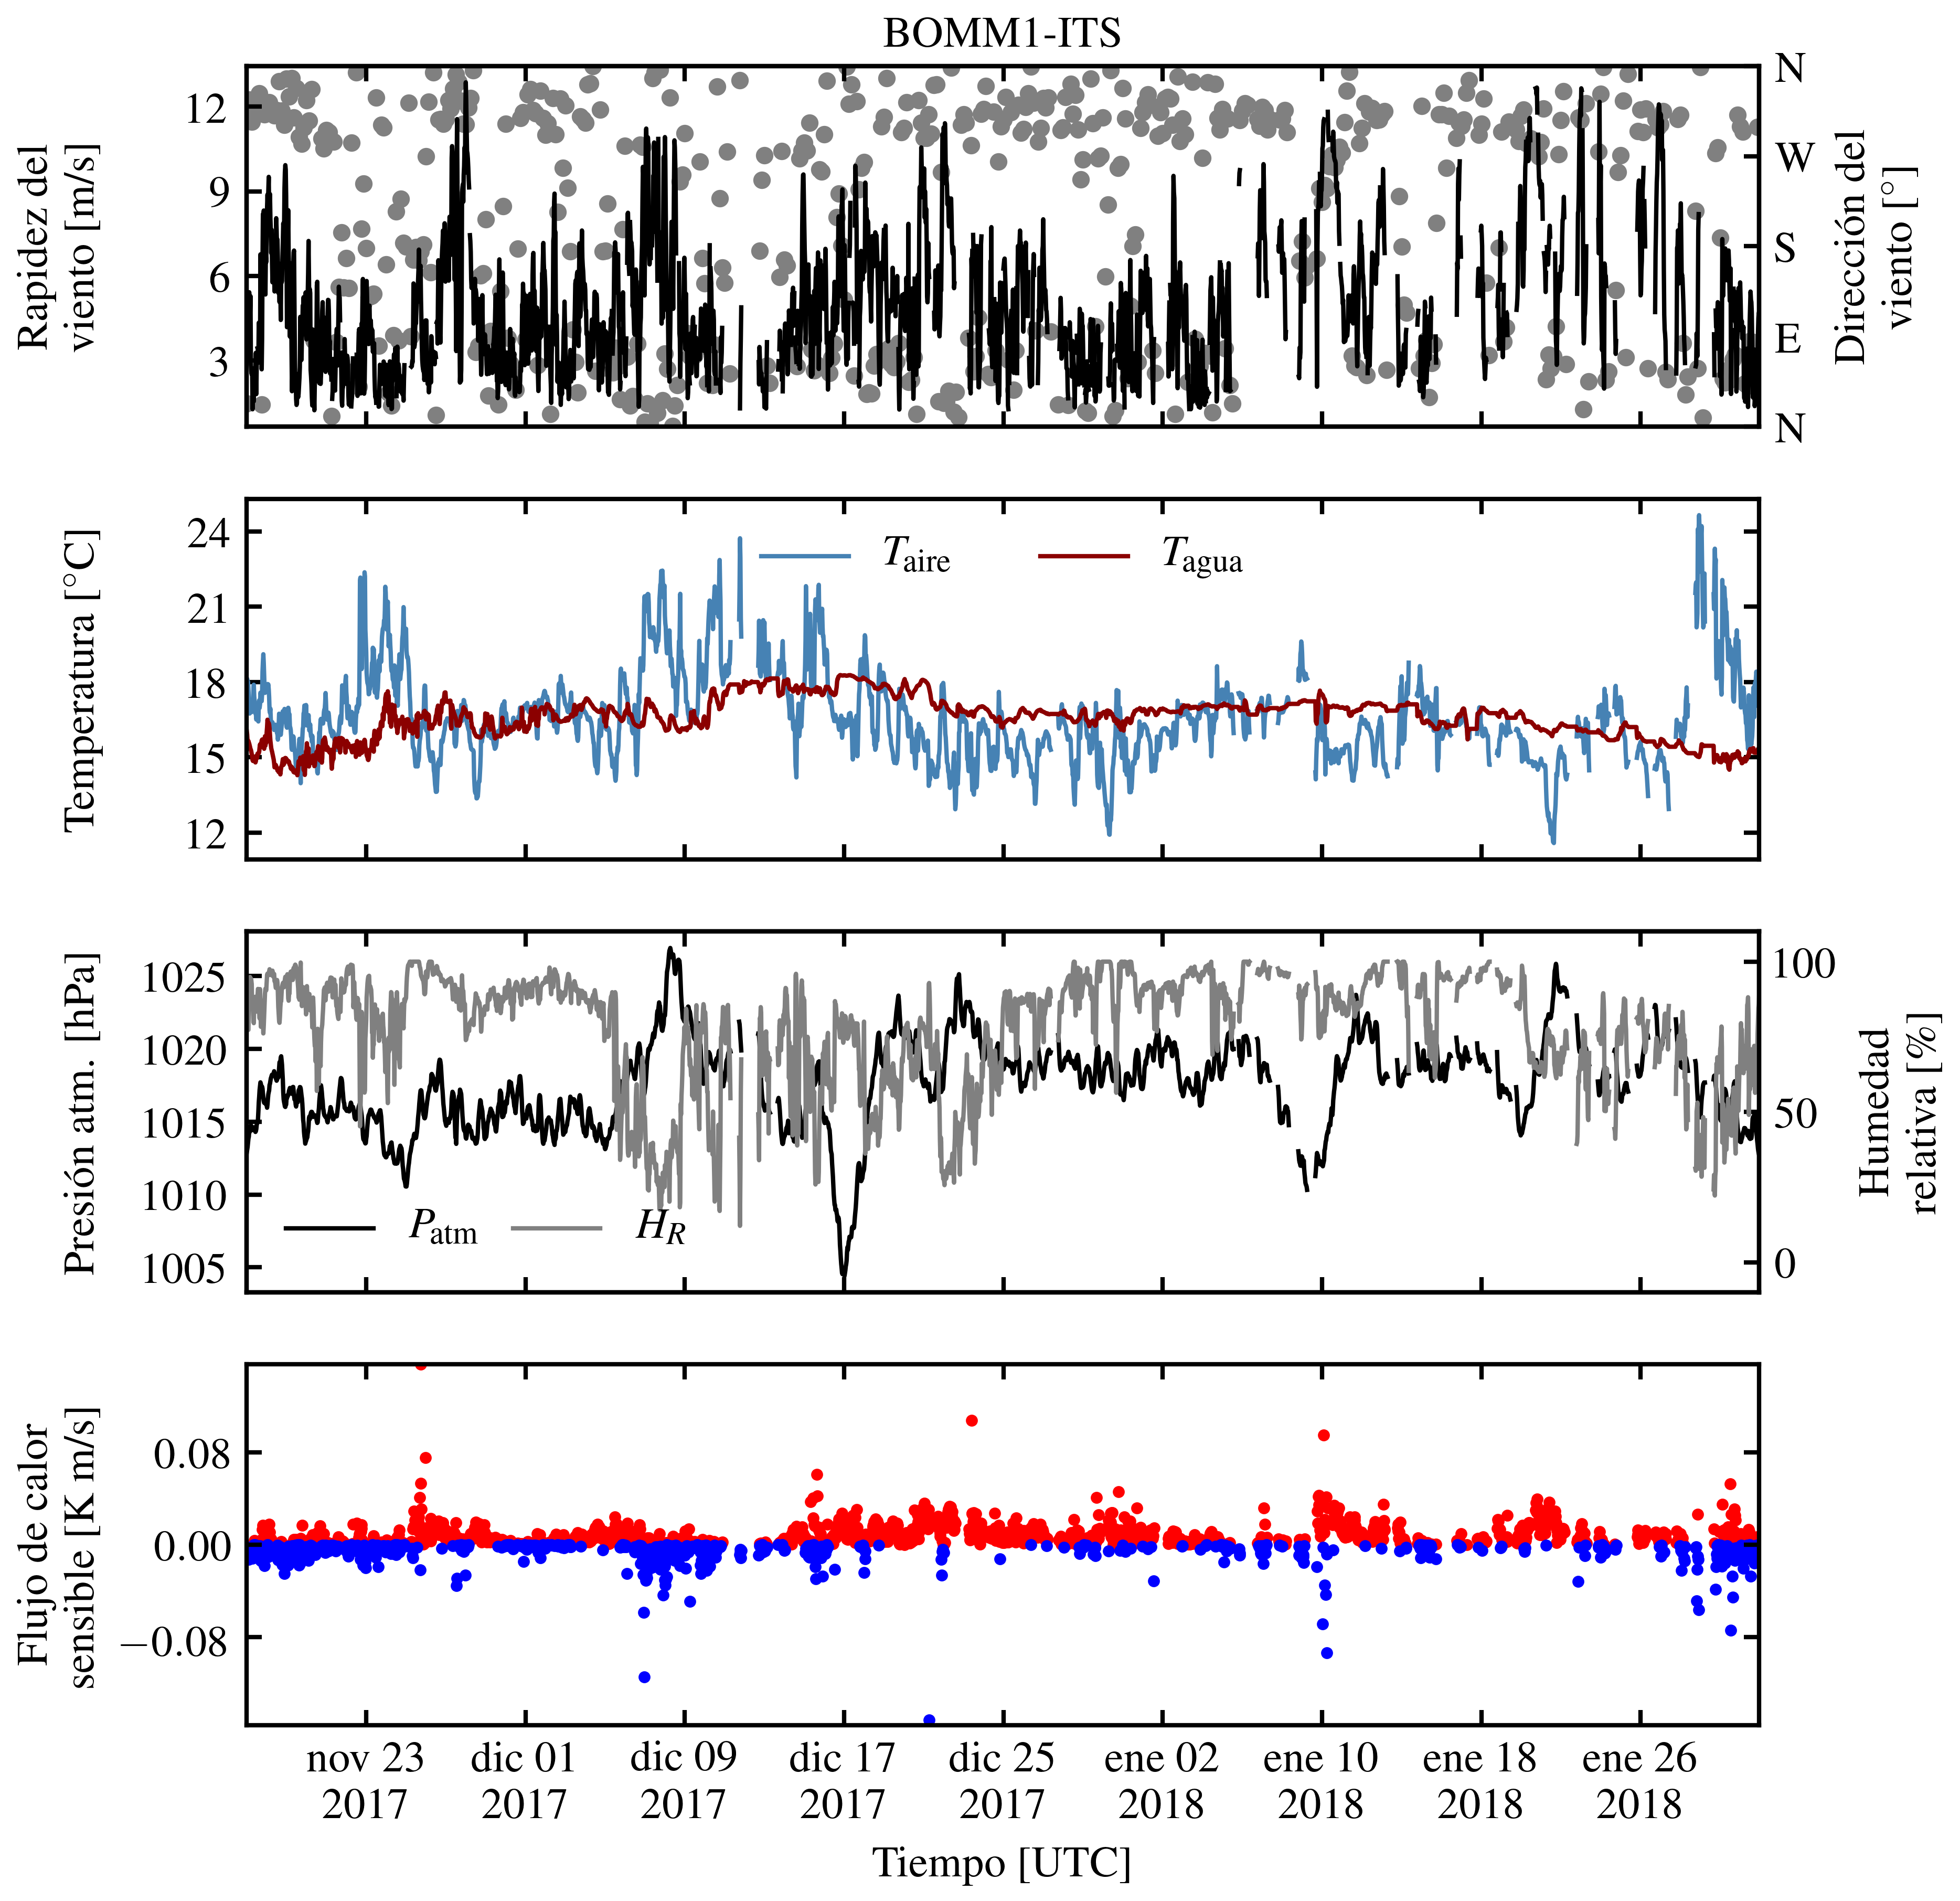
\includegraphics[width=0.85\linewidth]{../figures/bomm1_its_main_variables.png}
  \caption{
    Series de tiempo de las principales variables atmosféricas medidas durante
    el experimento BOMM1-ITS en las inmediaciones de la Isla Todos Santos,
    Ensenada, BC.
  }
  \label{fig:bomm1_its_main_variables}
\end{figure}

Durante el período de mediación de esta boya, se observaron vientos con una
rapidez entre 0 y 12 m/s y una dirección predominantemente del norte-noroeste.
Se logró observar el efecto que tiene los vientos de Santa Ana: cuando se
presentan estos eventos la dirección del viento es de tierra a mar, por lo tanto
se presentan unas bajas considerables en la humedad relativa (hasta un 30\%) y
una presión atmosférica promedio que supera los 1025 hPa. Adicionalmente,
durante estos eventos es evidente que el sentido del flujo de calor es
predominantemente de la atmósfera al océano, por lo tanto se observan
temperaturas del aire mayores que en el agua.

En la Figura \ref{fig:bomm1_its_wave_parameters} se presentan los principales
parámetros integrales del oleaje calculados a partir de las observaciones de los
alambres de capacitancia y el sensor de movimiento. Usando el método WDM
(Wavelet Directional Method) propuesto por \citet{Donelan1996}, se calculó el
espectro direccional del oleaje (ver reporte adjunto), del cual se derivan los
parámetros integrales del oleaje, que son, altura de ola significante (panel
superior) y período asociado al pico espectral (segundo panel). Adicionalmente
se presenta la rapidez del viento a 10 metros en condiciones neutrales (tercer
panel) y el espectro del oleaje en función de la frecuencia (panel inferior).

\begin{figure}[htpb]
  \centering
  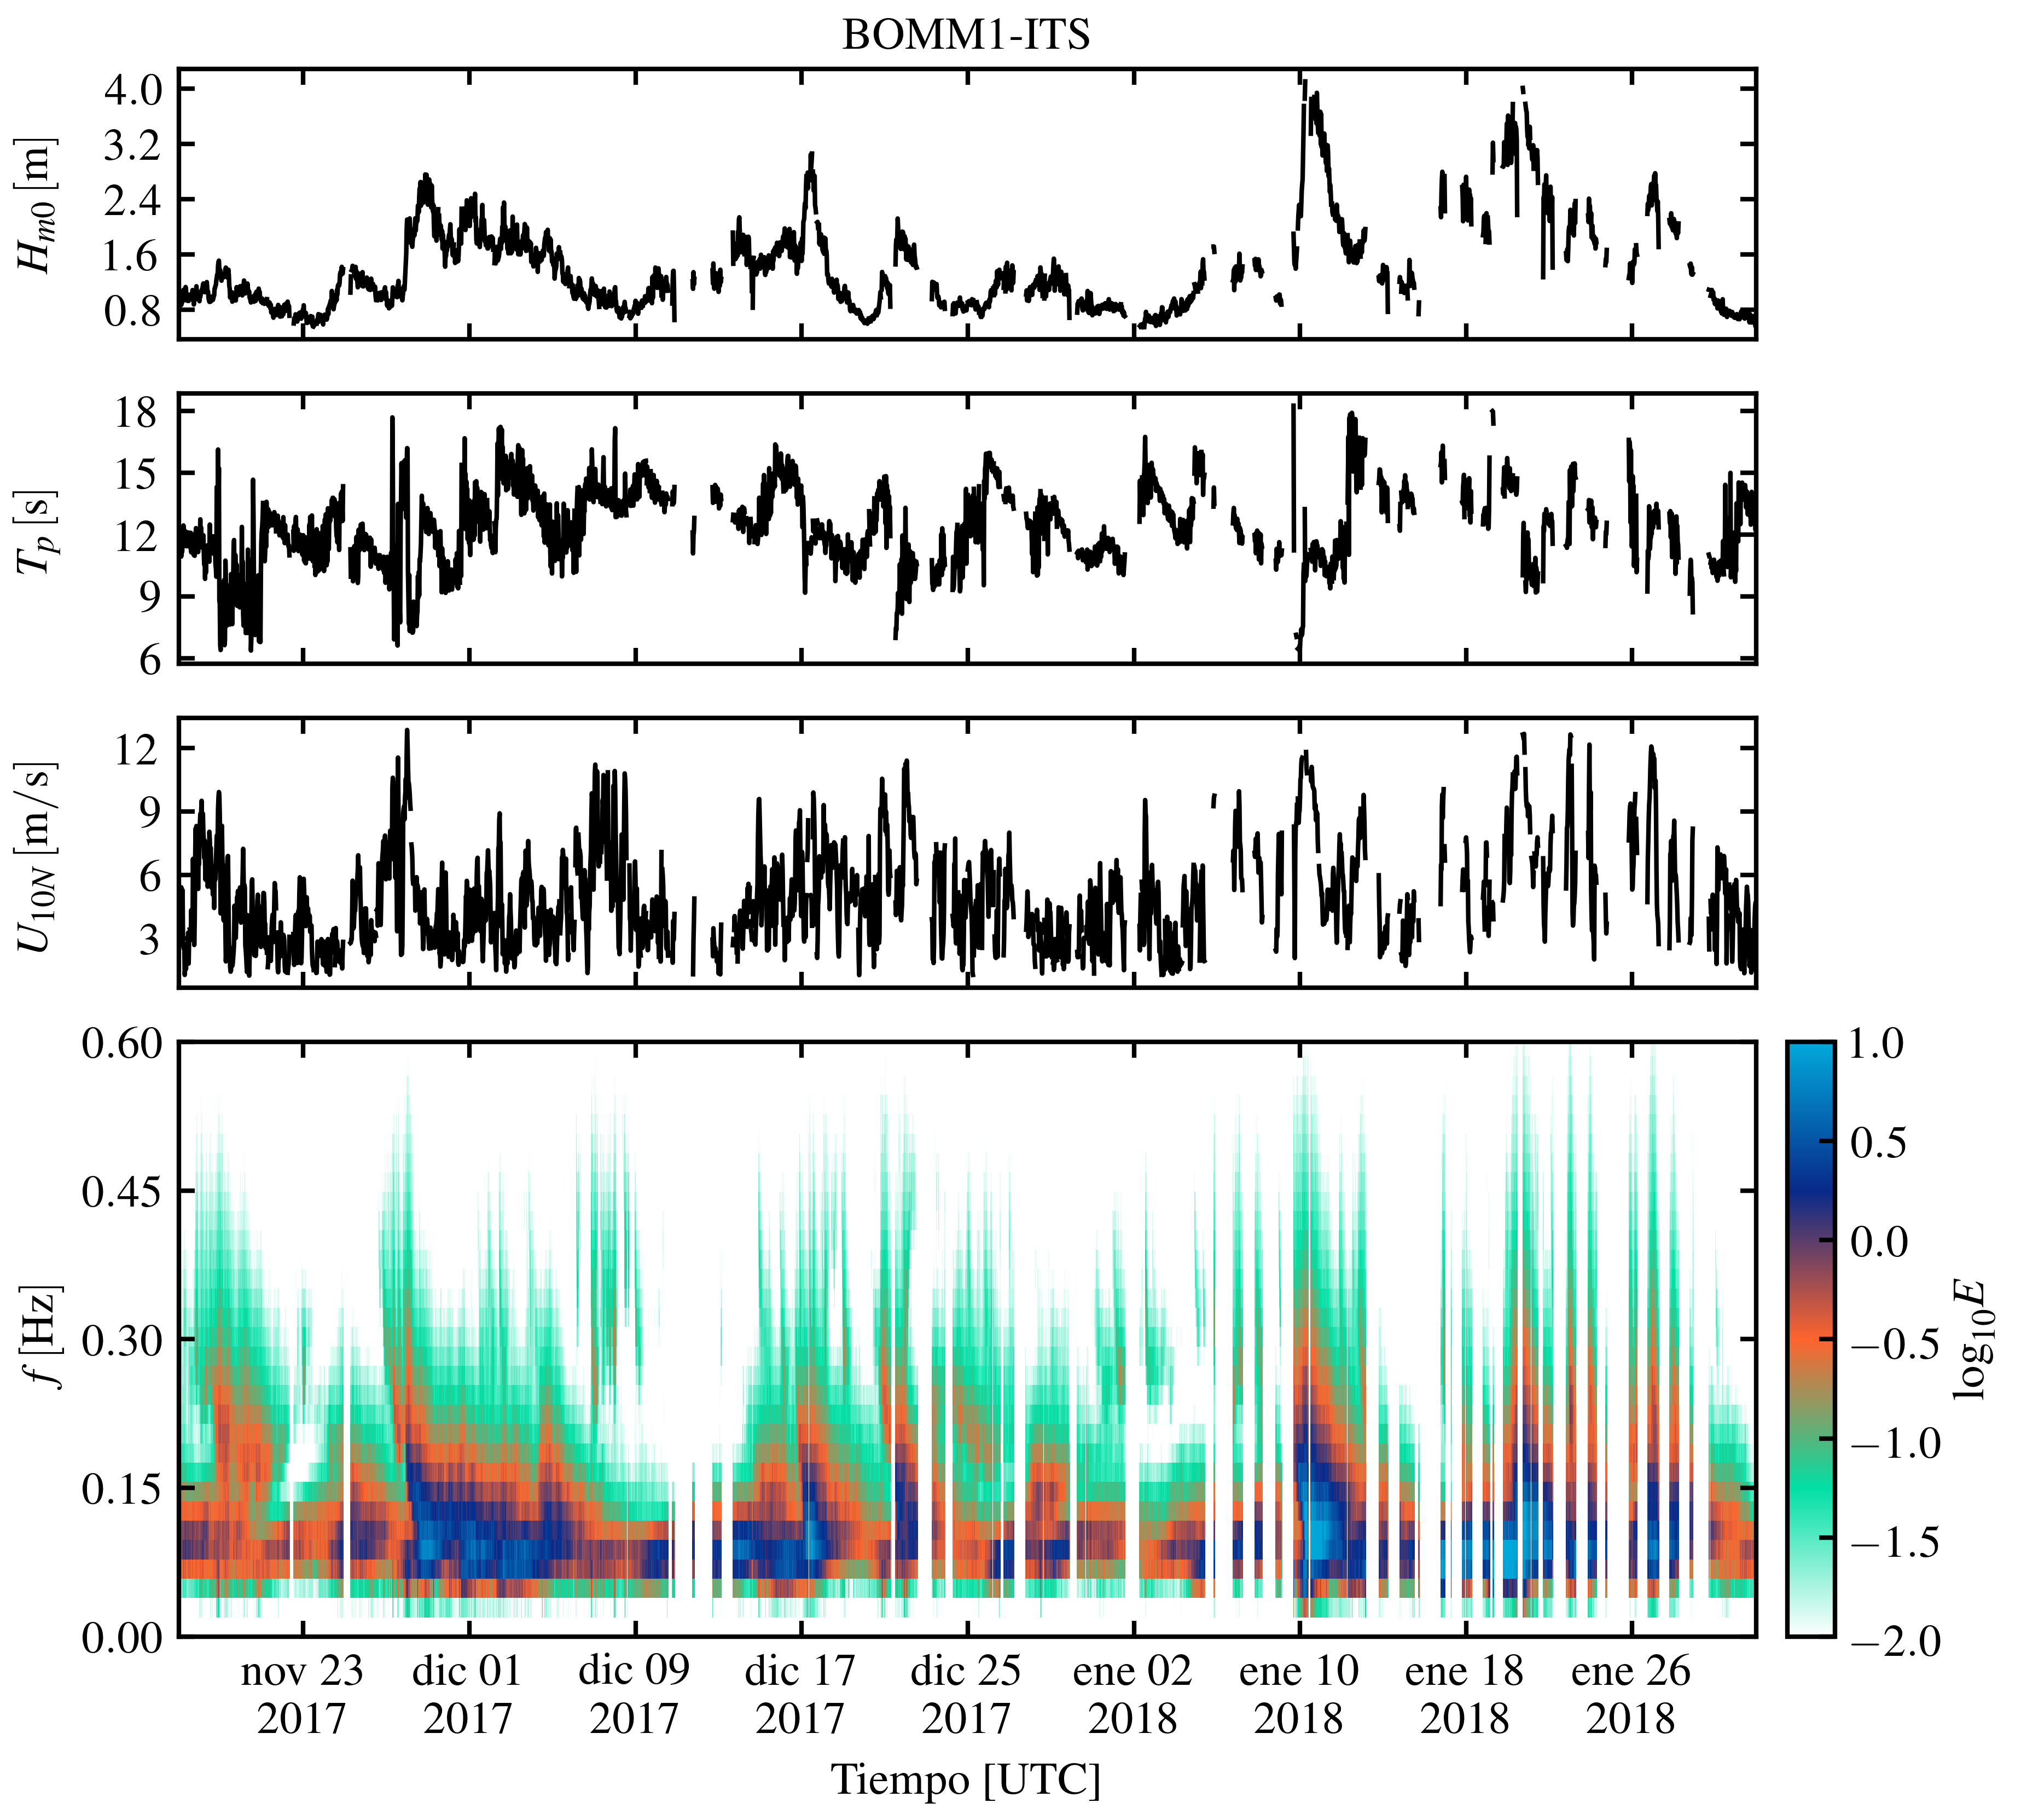
\includegraphics[width=0.85\linewidth]{../figures/bomm1_its_wave_parameters.png}
  \caption{
    Series de tiempo de algunas variables asociadas con el oleaje observadas el
    experimento BOMM1-ITS en las inmediaciones de la Isla Todos Santos,
    Ensenada, BC.
  }
  \label{fig:bomm1_its_wave_parameters}
\end{figure}

Se observaron alturas de significantes hasta de 4 m en algunos eventos. En esta
zona la mayor parte del tiempo se presentan condiciones de swell, por lo tanto
los períodos de las olas son generalmente mayores a 13 s, excepto en los casos
donde se presentan eventos de olas generadas casi-localmente o cercanas al punto
de medición, en los cuales los períodos son del orden de 6 a 9 s, junto con una
rapidez del viento mayor a 9 m/s.

Uno de los parámetros más importantes en la interacción océano-atmósfera es el
coeficiente de arrastre $C_D$. Este parámetro es una medida del momentum que se
transfiere de la atmósfera al océano. Muchos autores han propuesto
parametrizaciones del coeficiente de arrastre. En la Figura
\ref{fig:bomm1_its_drag_coefficient} se presentan los resultados obtenidos
durante el período de medición de la BOMM1 y se comparan con las curvas
propuestas por \citet{Smith1980} y por \citet{LargePond1981}. De manera general
se observa que, durante condiciones de vientos moderados a intensos, a medida
que aumenta la rapidez del viento, el coeficiente de arrastre aumenta
linealmente, pero cuando se presentan condiciones de viento ligero, hay un
aumento del coeficiente de arrastre a medida que el viento se acerca a cero.
Otro punto importante que se observó con las mediciones de la boya, es el efecto
que tiene el oleaje en el coeficiente de arrastre: como se observa en la figura,
el coeficiente de arrastre aumenta cuando aumenta la altura significante.

\begin{figure}[htpb]
  \centering
  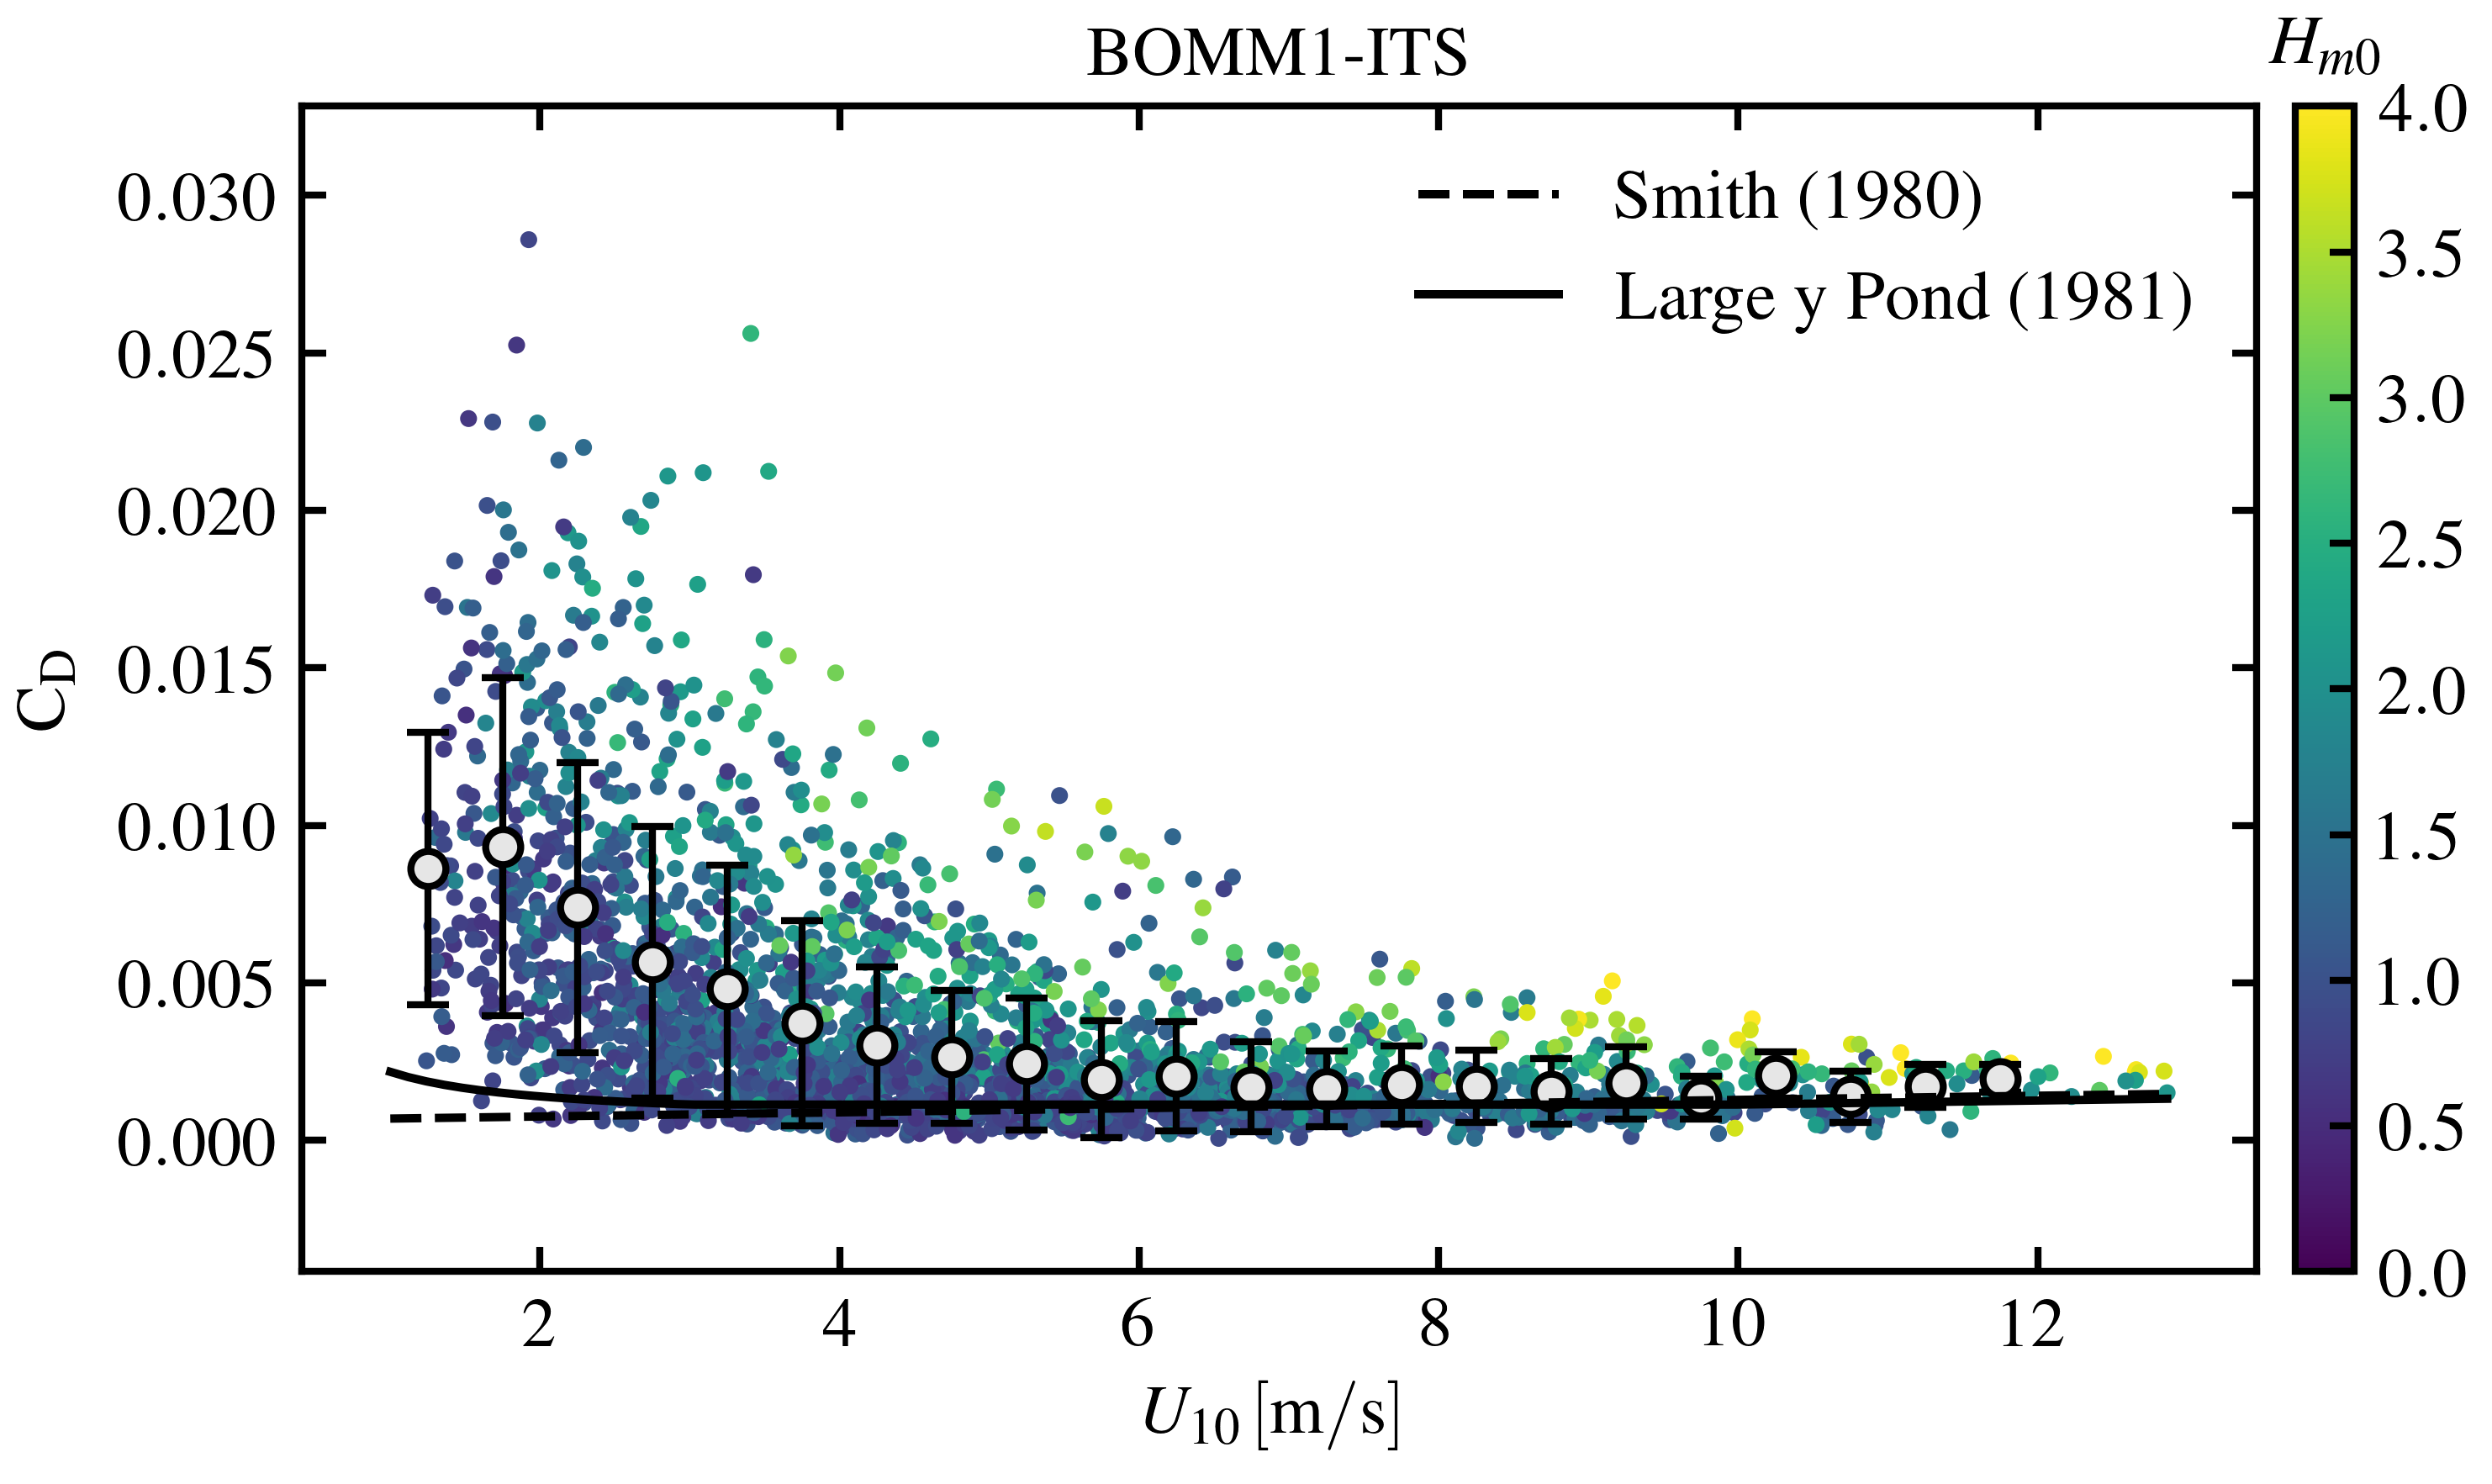
\includegraphics[width=0.68\linewidth]{../figures/bomm1_its_drag_coefficient.png}
  \caption{
    Coeficiente de arrastre en función de la rapidez del viento a 10 metros en
    condiciones neutrales observada durante el experimento BOMM1-ITS en las
    inmediaciones de la Isla Todos Santos, Ensenada, BC.  La barra de colores
    muestra la altura de ola significante como indicador del efecto de las olas
    en el coeficiente de arrastre. Las líneas sólida y punteada representan las
    parametrizaciones de \citet{Smith1980} y \citet{LargePond1981},
    respectivamente. Los puntos blancos con borde negro representan los
    promedios de $C_D$ para 20 intervalos de clase de $U_{10}$ y las barras
    representan la desviación estándar de cada intervalo.
  }
  \label{fig:bomm1_its_drag_coefficient}
\end{figure}

Pueden existir diferencias entre la dirección del viento real obtenida de la
Maximet\footnote{real quiere decir la dirección del viento relativa al norte
magnético} y la dirección que se obtiene del anemómetro sónico. En el segundo
caso la dirección del viento se obtiene a partir de la corrección de los datos
por el movimiento de la boya, lo cual incluye la orientación de la misma
respecto al norte magnético (ver reporte adjunto). En la Figura
\ref{fig:bomm1_its_wind_direction_histogram} se presenta un histograma de la
diferencia entre estos dos ángulos. Se espera que el valor más probable sea cero
y que haya una muy baja variabilidad. En el caso de la BOMM1-ITS se observa una
diferencia que oscila entre -10 y +10 grados, lo cual puede deberse a errores en
la corrección por el movimiento, desalineamientos entre los sensores o
diferencias reales en la dirección del viento debido a la distorsión del flujo
por la estructura.

\begin{figure}[htpb]
  \centering
  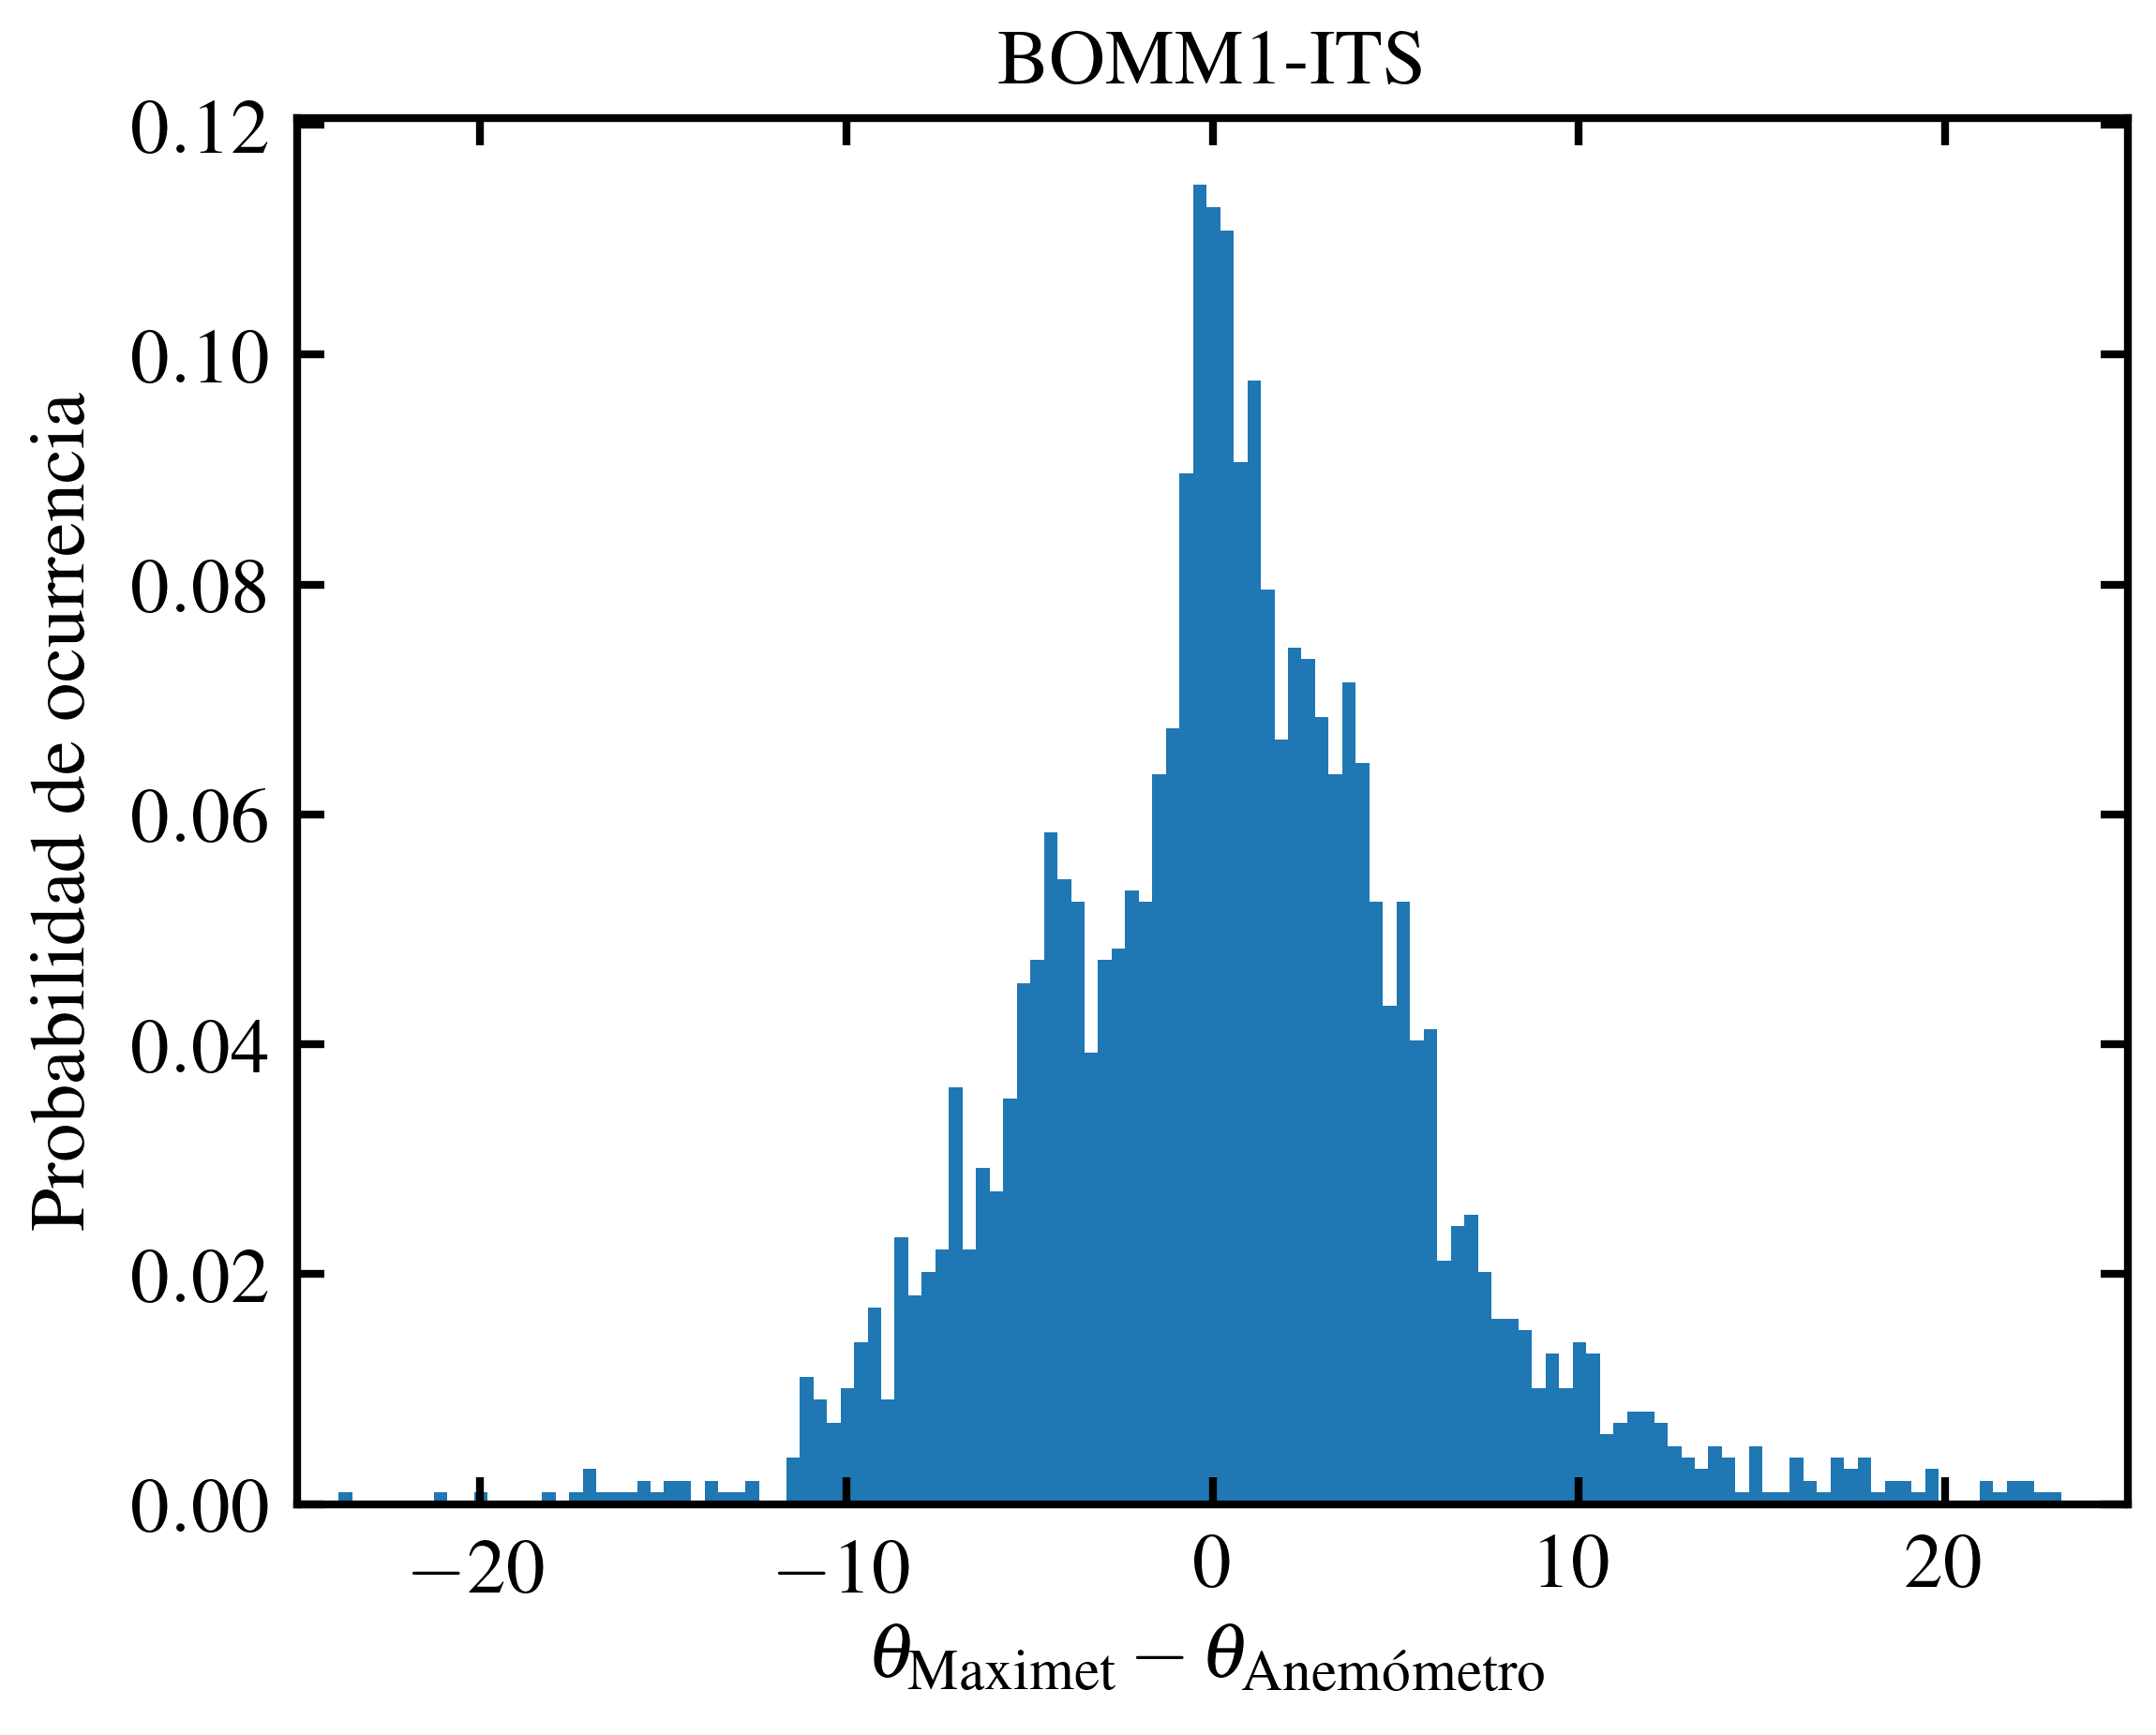
\includegraphics[width=0.5\linewidth]{../figures/bomm1_its_wind_direction_histogram.png}
  \caption{
    Histograma de la diferencia entre la dirección del viento real observada con
    la estación meteorológica Maximet y la dirección del viento calculada del
    anemómetro sónico después de aplicar la corrección de los datos por el
    movimiento de la boya. Los datos corresponden a las observaciones llevadas a
    cabo durante el experimento BOMM1-ITS en las inmediaciones de la Isla Todos
    Santos, Ensenada, BC.
  }
  \label{fig:bomm1_its_wind_direction_histogram}
\end{figure}


% }}}

% bomm2-its {{{
\subsection{BOMM2-ITS}
\label{sub:bomm2_its}

La BOMM2-ITS fue la segunda boya que se construyó. El experimento en ITS se
llevó a cabo entre el 2018/03/03 y el 2018/06/19 y se midieron las mismas
variables que en el caso anterior. En este caso se tiene un mayor período de
medición que durante el experimento BOMM1-ITS y a diferencia de aquel, en este
caso se observó el período de transición entre primavera y principios del verano
(Figura \ref{fig:bomm2_its_main_variables}). Esto se ve claramente en el aumento
gradual de la temperatura subsuperficial del mar que se da desde finales de mayo
hasta el final del período de medición acompañado por una disminución de la
presión atmosférica.  Durante este tiempo la rapidez del viento osciló entre 0 y
11 m/s e igualmente las direcciones predominantes fueron del norte-noroeste. Se
logran observar dos eventos de vientos de Santa Ana en los meses de marzo y
abril, en donde la temperatura del aire fue casi dos veces la temperatura del
aire, por lo tanto se observaron unos flujos de calor sensible considerablemente
intensos comparados con el caso de la BOMM1-ITS.

\begin{figure}[htpb]
  \centering
  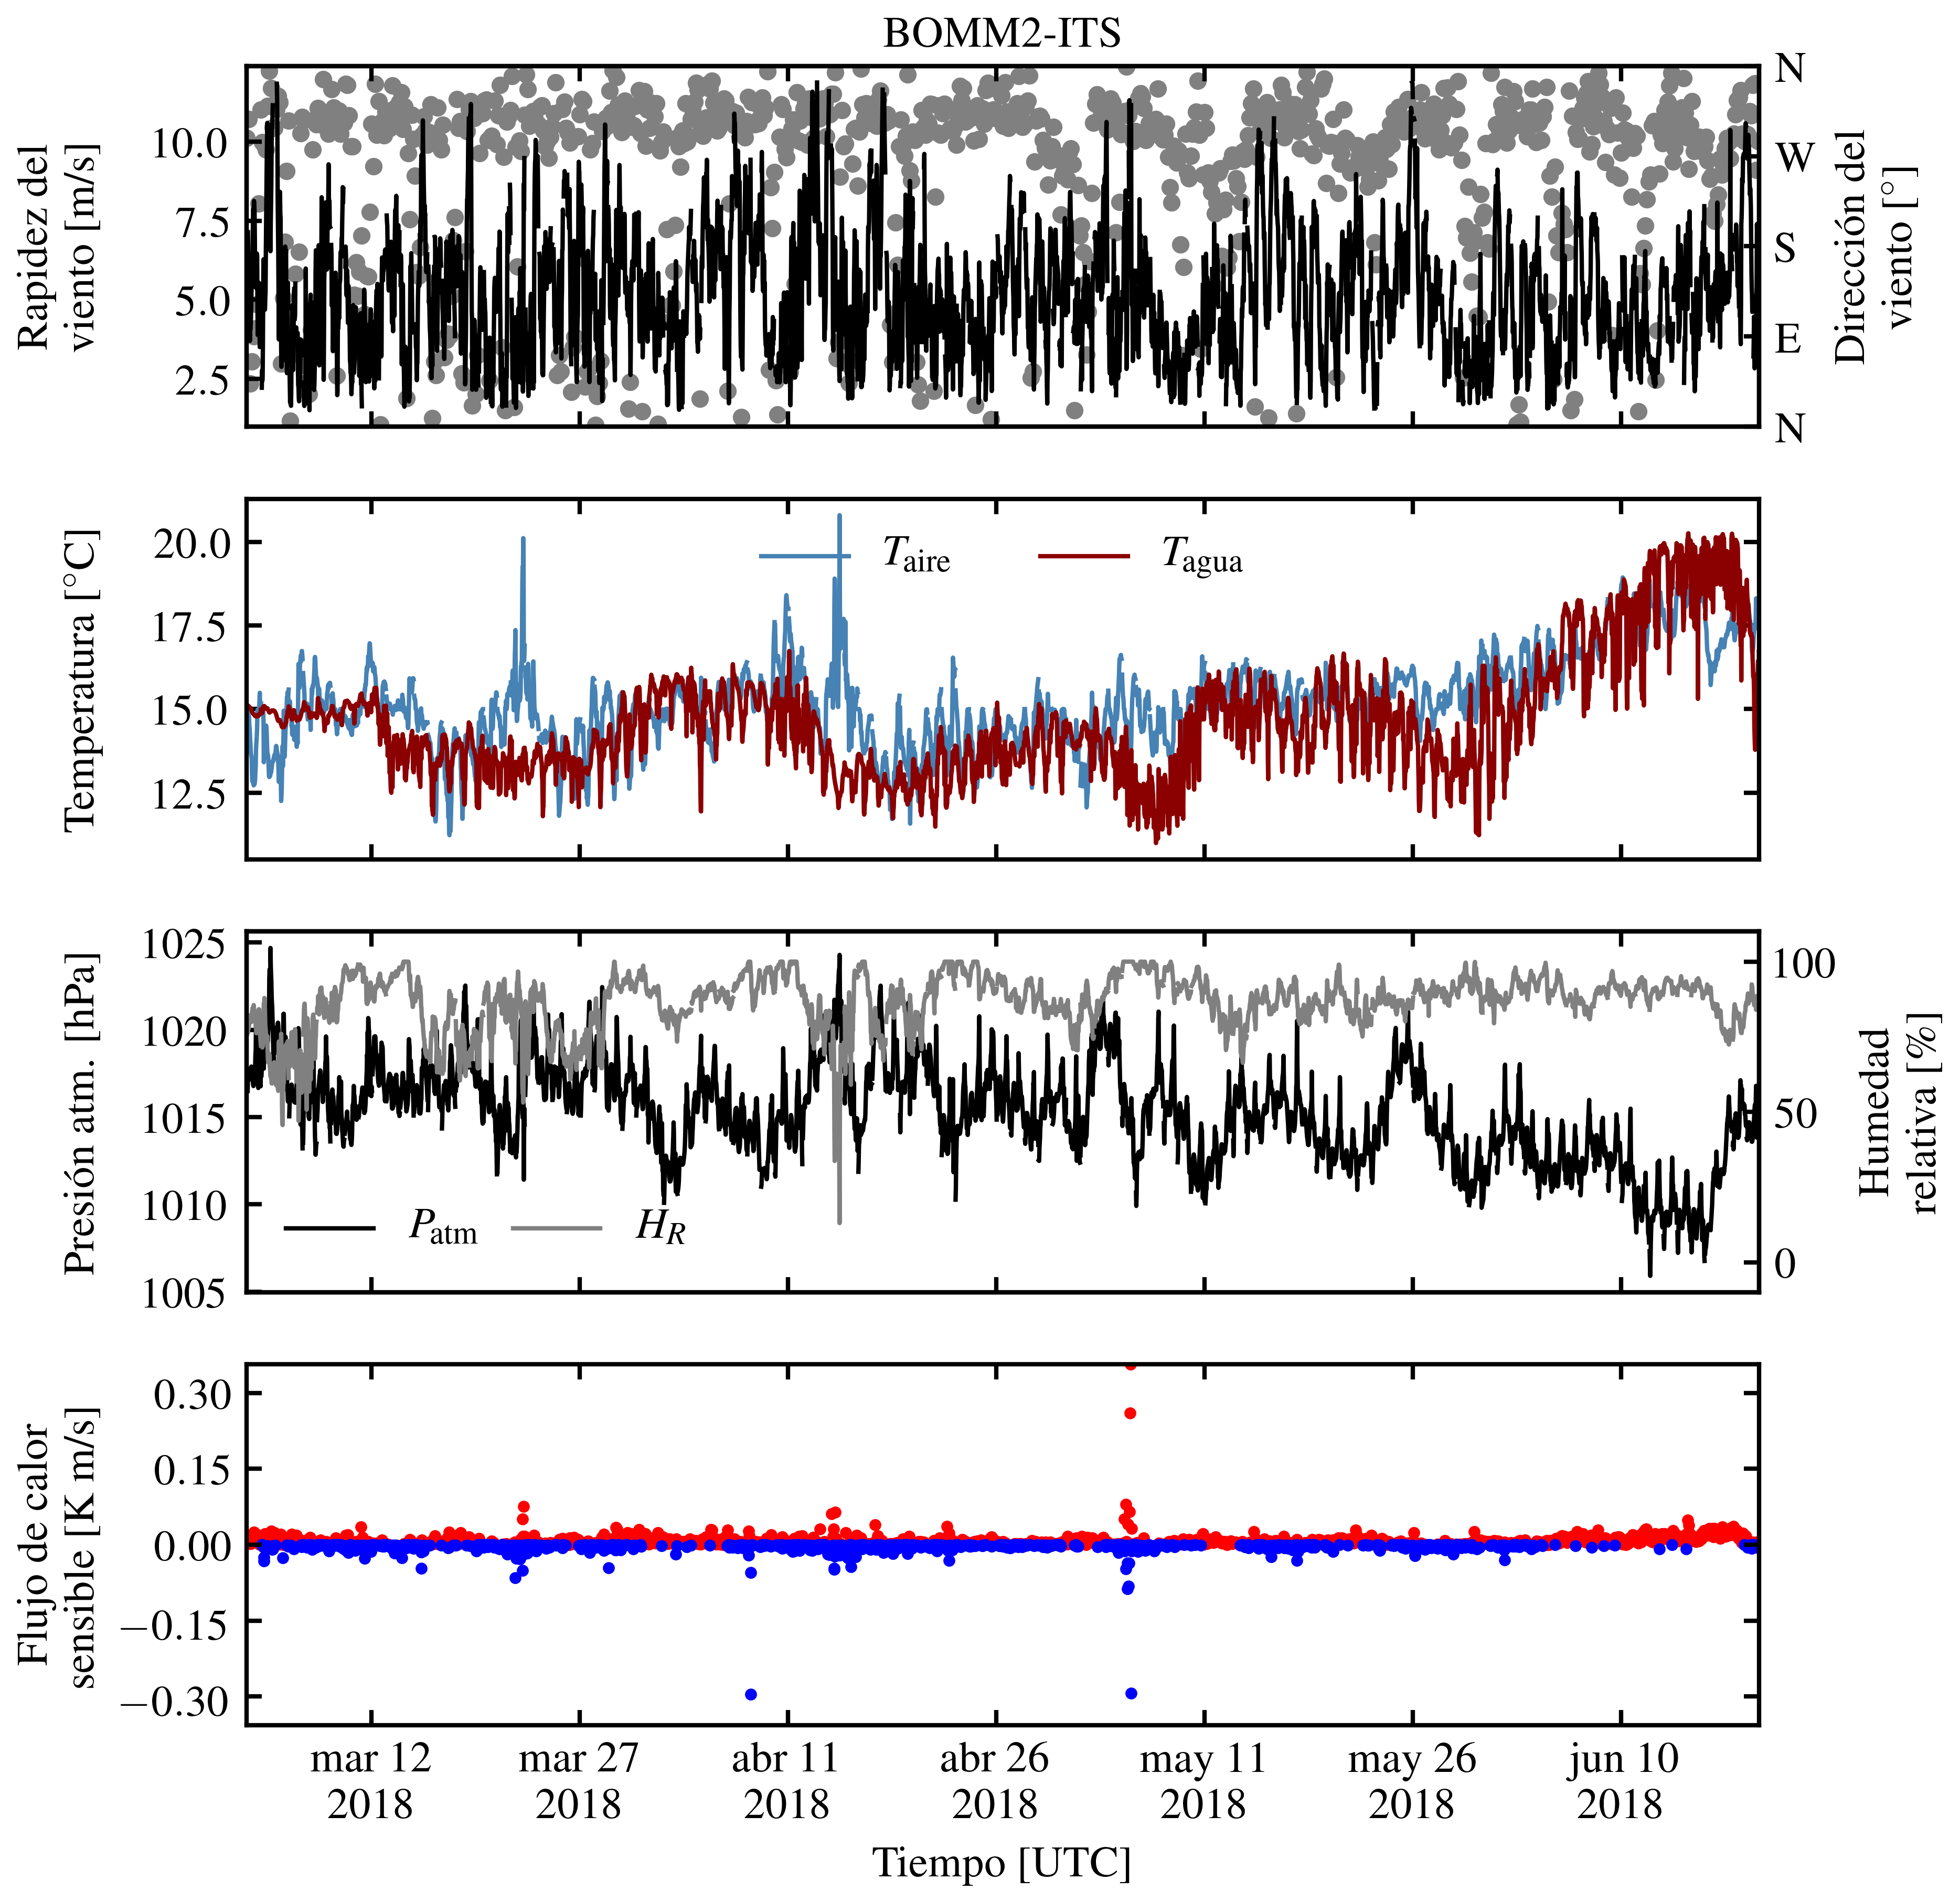
\includegraphics[width=0.85\linewidth]{../figures/bomm2_its_main_variables.png}
  \caption{
    Series de tiempo de las principales variables atmosféricas medidas durante
    el experimento BOMM2-ITS en las inmediaciones de la Isla Todos Santos,
    Ensenada, BC.
  }
  \label{fig:bomm2_its_main_variables}
\end{figure}

En el caso de los parámetros del oleaje se observaron alturas de ola menores que
en período anterior ya que corresponden a los meses de primavera y verano. En
cuanto al período del pico espectral, los valores oscilan igualmente entre 6 y
18 s, En el espectro en frecuencia de este período en particular, se logra
observar el arribo de sistemas de swell como franjas azules con cierta
pendiente, lo cual es un proceso que se conoce como dispersión del oleaje, y es
consecuencia de que las olas más largas viajan más rápido que las corta, por lo
tanto primero se observan ondas de menor frecuencia y esta aumenta conforme pasa
el tiempo (Figura \ref{fig:bomm2_its_wave_parameters}).

\begin{figure}[htpb]
  \centering
  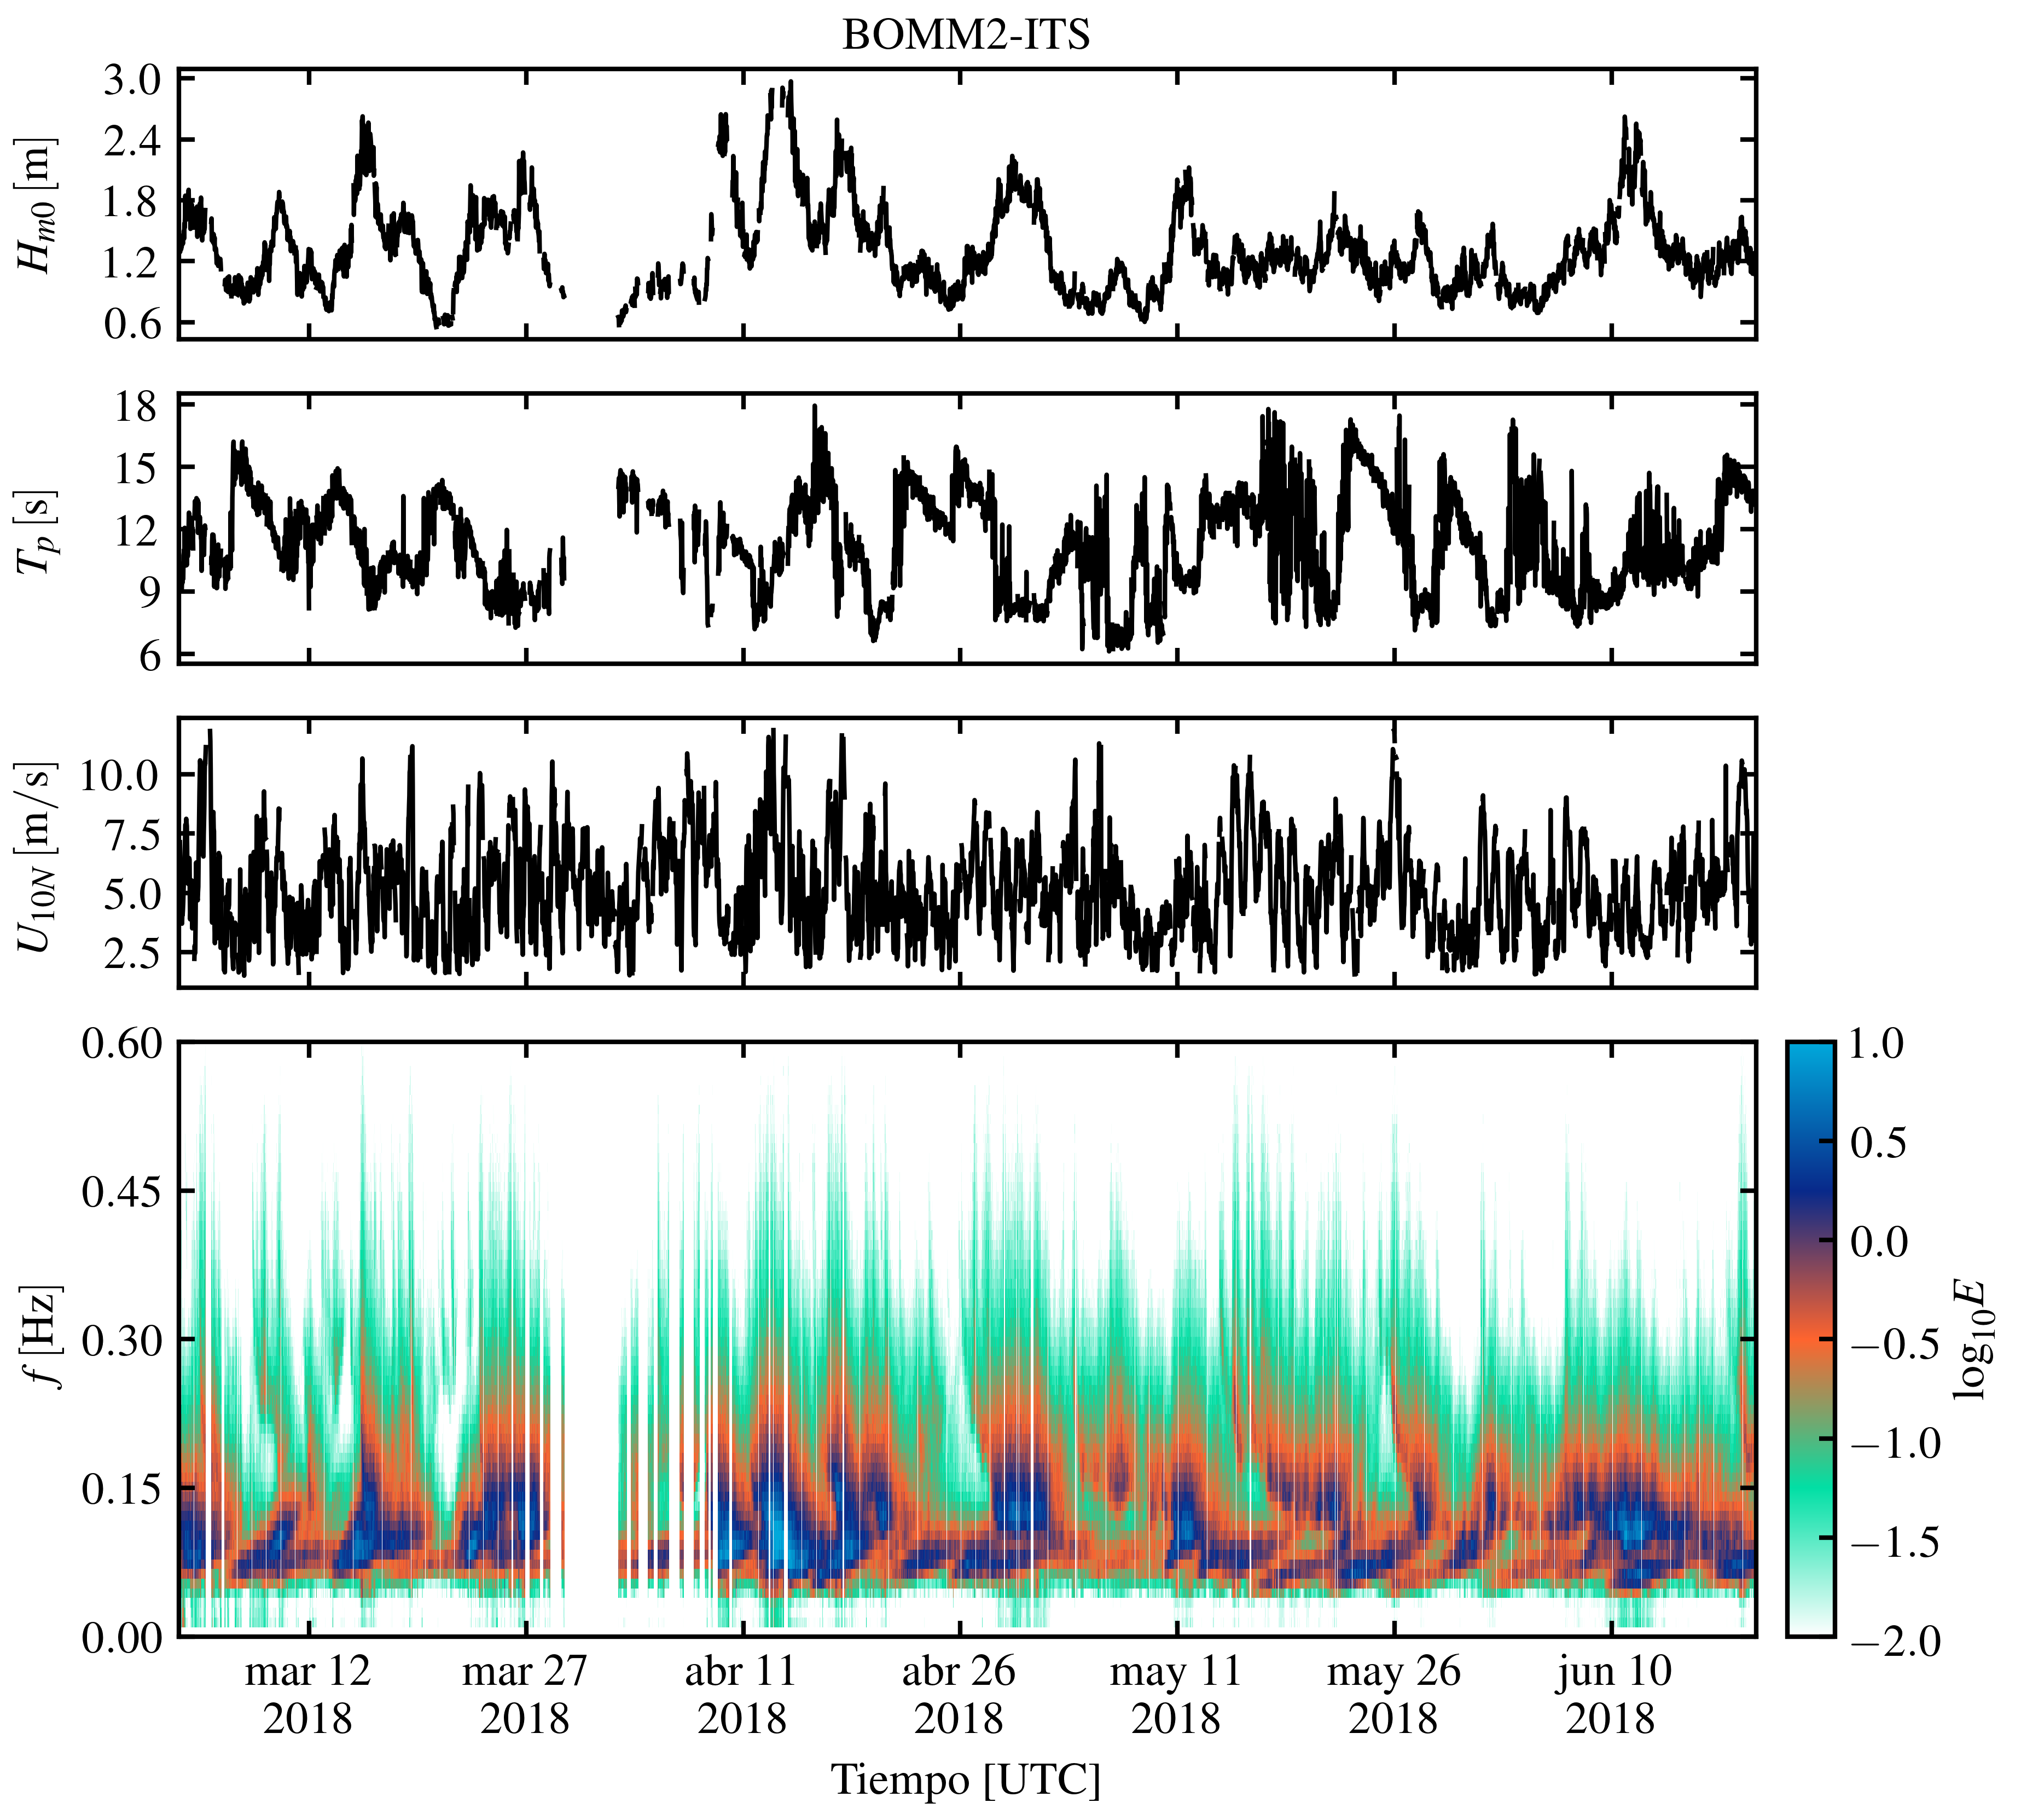
\includegraphics[width=0.85\linewidth]{../figures/bomm2_its_wave_parameters.png}
  \caption{
    Series de tiempo de algunas variables asociadas con el oleaje observadas el
    experimento BOMM2-ITS en las inmediaciones de la Isla Todos Santos,
    Ensenada, BC.
  }
  \label{fig:bomm2_its_wave_parameters}
\end{figure}

Al igual que durante el período de medición de la BOMM1-ITS, el coeficiente de
arrastre presenta el mismo comportamiento en lo que se observó durante el
experimento BOMM2-ITS, como se muestra en la Figura
\ref{fig:bomm2_its_drag_coefficient}. Cabe mencionar que en este caso, el efecto
del aumento del coeficiente de arrastre por cuenta del aumento de la altura
significante del oleaje, no se observa tan claro, posiblemente debido a que
durante el período de la BOMM2-ITS no se alcanzaron las alturas de ola
registradas durante el experimento de la BOMM1-ITS.

\begin{figure}[htpb]
  \centering
  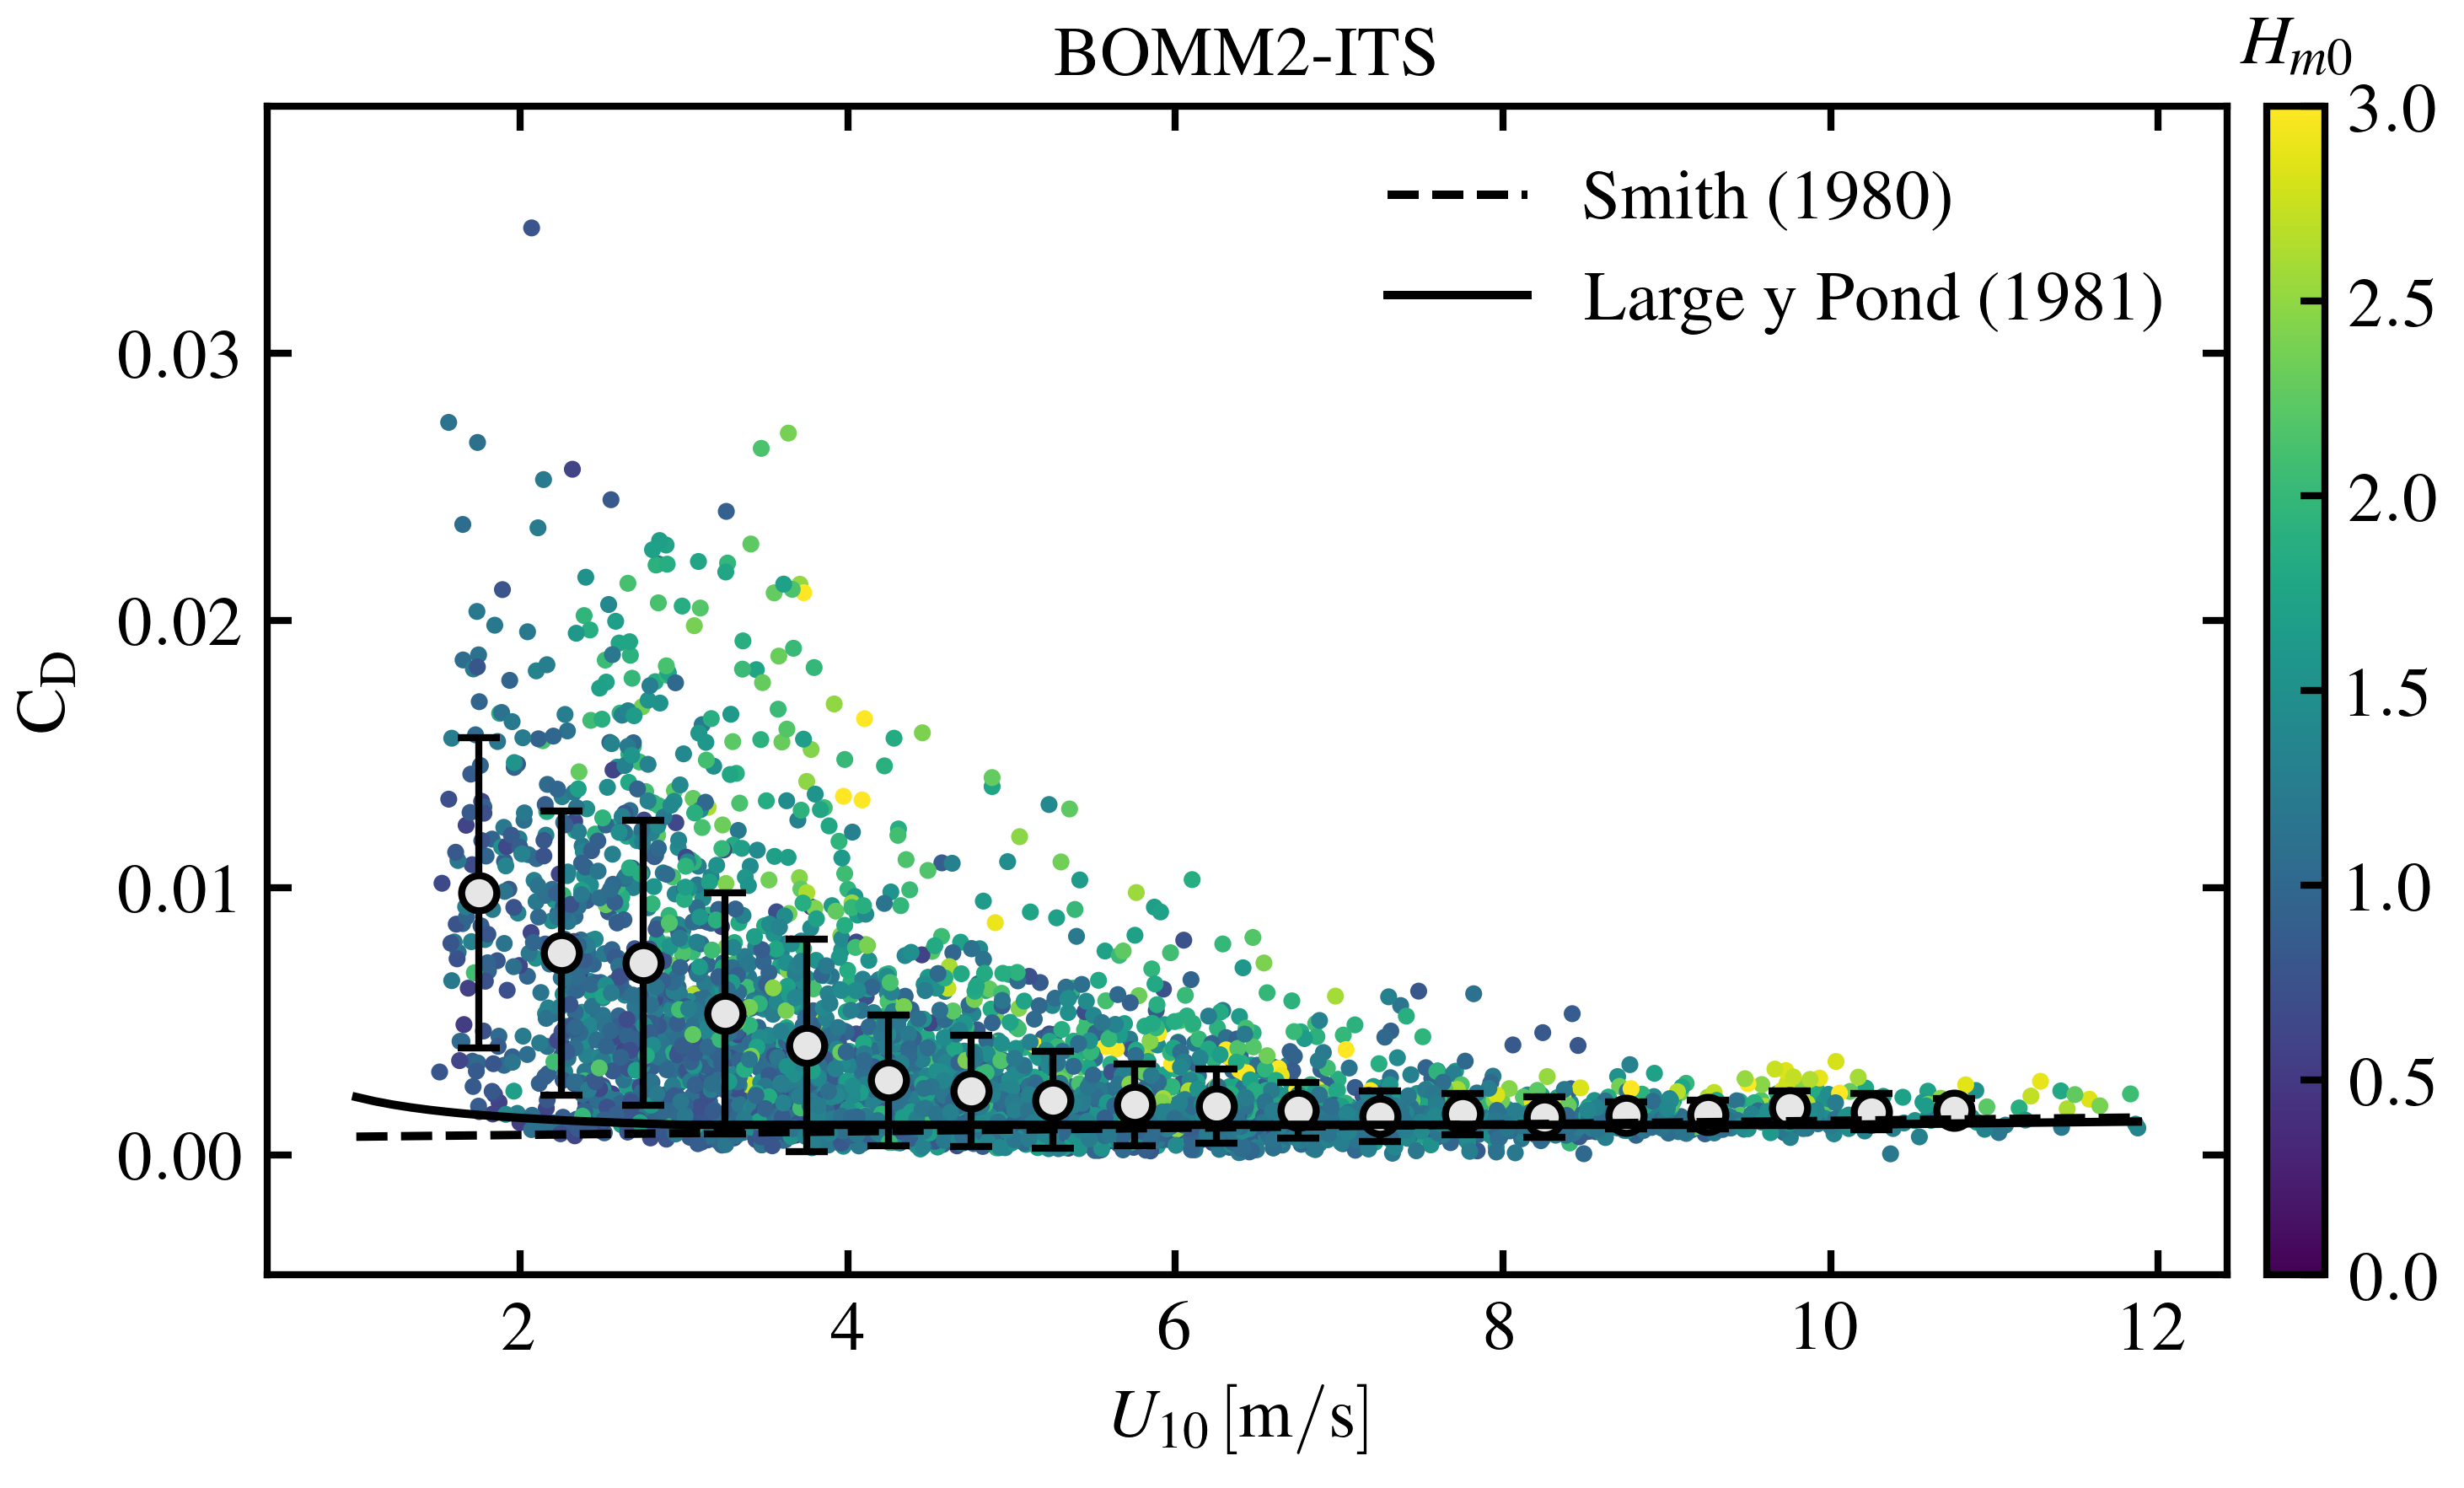
\includegraphics[width=0.68\linewidth]{../figures/bomm2_its_drag_coefficient.png}
  \caption{
    Coeficiente de arrastre en función de la rapidez del viento a 10 metros en
    condiciones neutrales observada durante el experimento BOMM1-ITS en las
    inmediaciones de la Isla Todos Santos, Ensenada, BC.  La barra de colores
    muestra la altura de ola significante como indicador del efecto de las olas
    en el coeficiente de arrastre. Las líneas sólida y punteada representan las
    parametrizaciones de \citet{Smith1980} y \citet{LargePond1981},
    respectivamente. Los puntos blancos con borde negro representan los
    promedios de $C_D$ para 20 intervalos de clase de $U_{10}$ y las barras
    representan la desviación estándar de cada intervalo.
  }
  \label{fig:bomm2_its_drag_coefficient}
\end{figure}

Finalmente, en la figura que muestra la diferencia entre la dirección del viento
obtenida de la Maximet y la calculada a partir de las componentes de la
velocidad del anemómetro sónico después de aplicar la corrección por el
movimiento de la boya (Figura \ref{fig:bomm2_its_wind_direction_histogram}), se
puede observar un leve sesgo entre 3 y 4 grados, aunque la dispersión de los
datos se encuentra entre -10 y +10, al igual que en la BOMM1-ITS.

\begin{figure}[htpb]
  \centering
  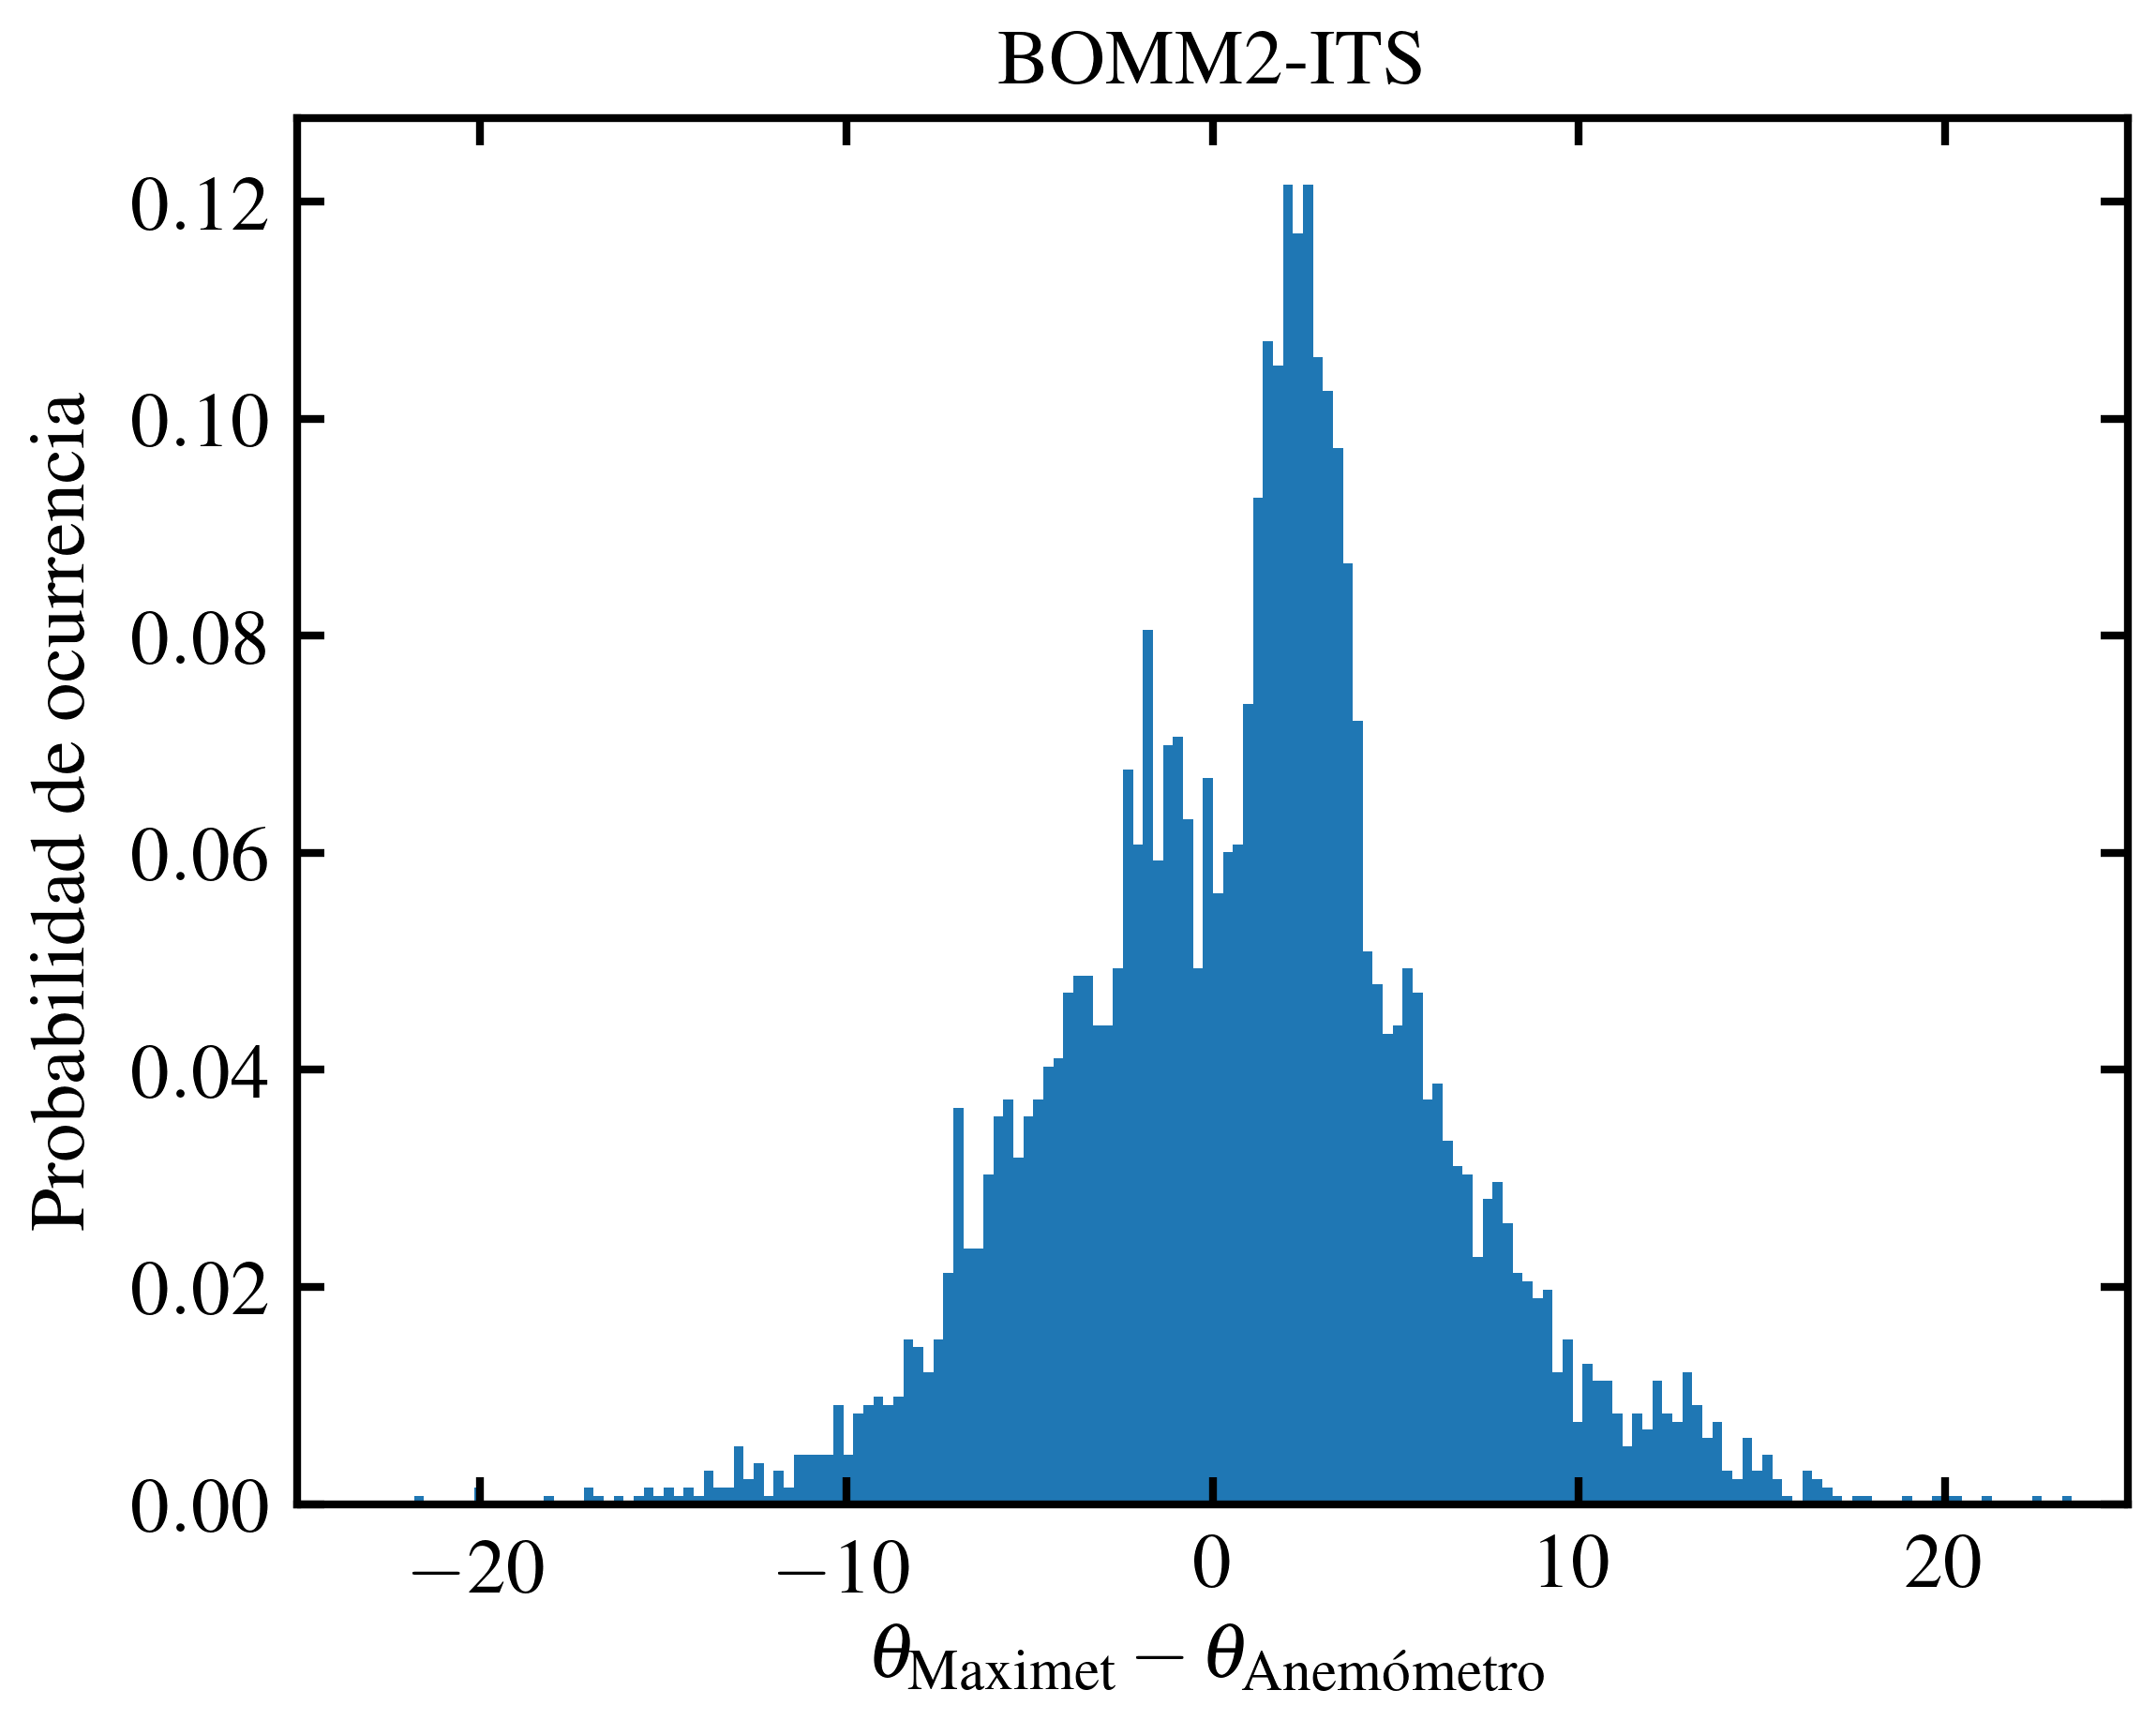
\includegraphics[width=0.5\linewidth]{../figures/bomm2_its_wind_direction_histogram.png}
  \caption{
    Histograma de la diferencia entre la dirección del viento real observada con
    la estación meteorológica Maximet y la dirección del viento calculada del
    anemómetro sónico después de aplicar la corrección de los datos por el
    movimiento de la boya. Los datos corresponden a las observaciones llevadas a
    cabo durante el experimento BOMM2-ITS en las inmediaciones de la Isla Todos
    Santos, Ensenada, BC.
  }
  \label{fig:bomm2_its_wind_direction_histogram}
\end{figure}
% }}}

% bomm1-per {{{
\subsection{BOMM1-PER}
\label{sub:bomm1_per}

Luego del período de pruebas en el punto ITS, la BOMM1 se instaló en Perdido
(Golfo de México). El período de medición abarcó desde el 2018/07/11 hasta el
2019/02/27. A continuación se presentan las gráficas que muestran los resultados
más relevantes obtenidos de las observaciones de la BOMM1-PER.  En la Figura
\ref{fig:bomm1_per_main_variables} presentan las principales variables
meteorológicas. Es importante notar la diferencia que existe entre las
condiciones atmosféricas y meteorológicas en Isla Todos Santos y en el Golfo de
México. Con el experimento BOMM1-PER se logró observar una alta variabilidad de
la rapidez del viento, oscilando entre 2 y 25 m/s. Las direcciones predominantes
observados son del sur-sureste en la temporada de julio a octubre y del
norte-noroeste en la temporada de noviembre a febrero. En este último período se
observan una cantidad considerable de eventos conocidos como ``Nortes'', los
cuales se caracterízan por una rapidez del viento que supera los 20 m/s,
acompañados por un descenso abrupto en la temperatura del aire, que en el caso
por ejemplo del evento de Norte de mediados del mes de octubre, pasó de $\sim
30^\circ\mathrm{C}$ a $\sim 18^\circ\mathrm{C}$ en poco menos de un día. Esta
reducción también estuvo acompañada de un descenso en la temperatura
subsuperficial del mar de casi $3^\circ\mathrm{C}$ y un aumento de la humedad
relativa hasta 95\%. Posterior a este evento, se puede observar un Norte a
mediados de noviembre de igual intensidad que el anterior, donde se alcanzaron
casi 25 m/s de rapidez del viento y se presentó un descenso en la temperatura
del aire hasta $12^\circ\mathrm{C}$. En este caso, la presión atmosférica
aumento considerablemente respecto a su promedio, superando los 1030 hPa. No se
cuenta con mediciones de temperatura del mar después de este evento debido a
problemas técnicos con el RBR. Los flujos de calor sensible durante los
``Norte'' son predominantemente positivos, es decir, del océano a la atmósfera,
lo cual es consecuente con las observaciones de temperatura.

\begin{figure}[htpb]
  \centering
  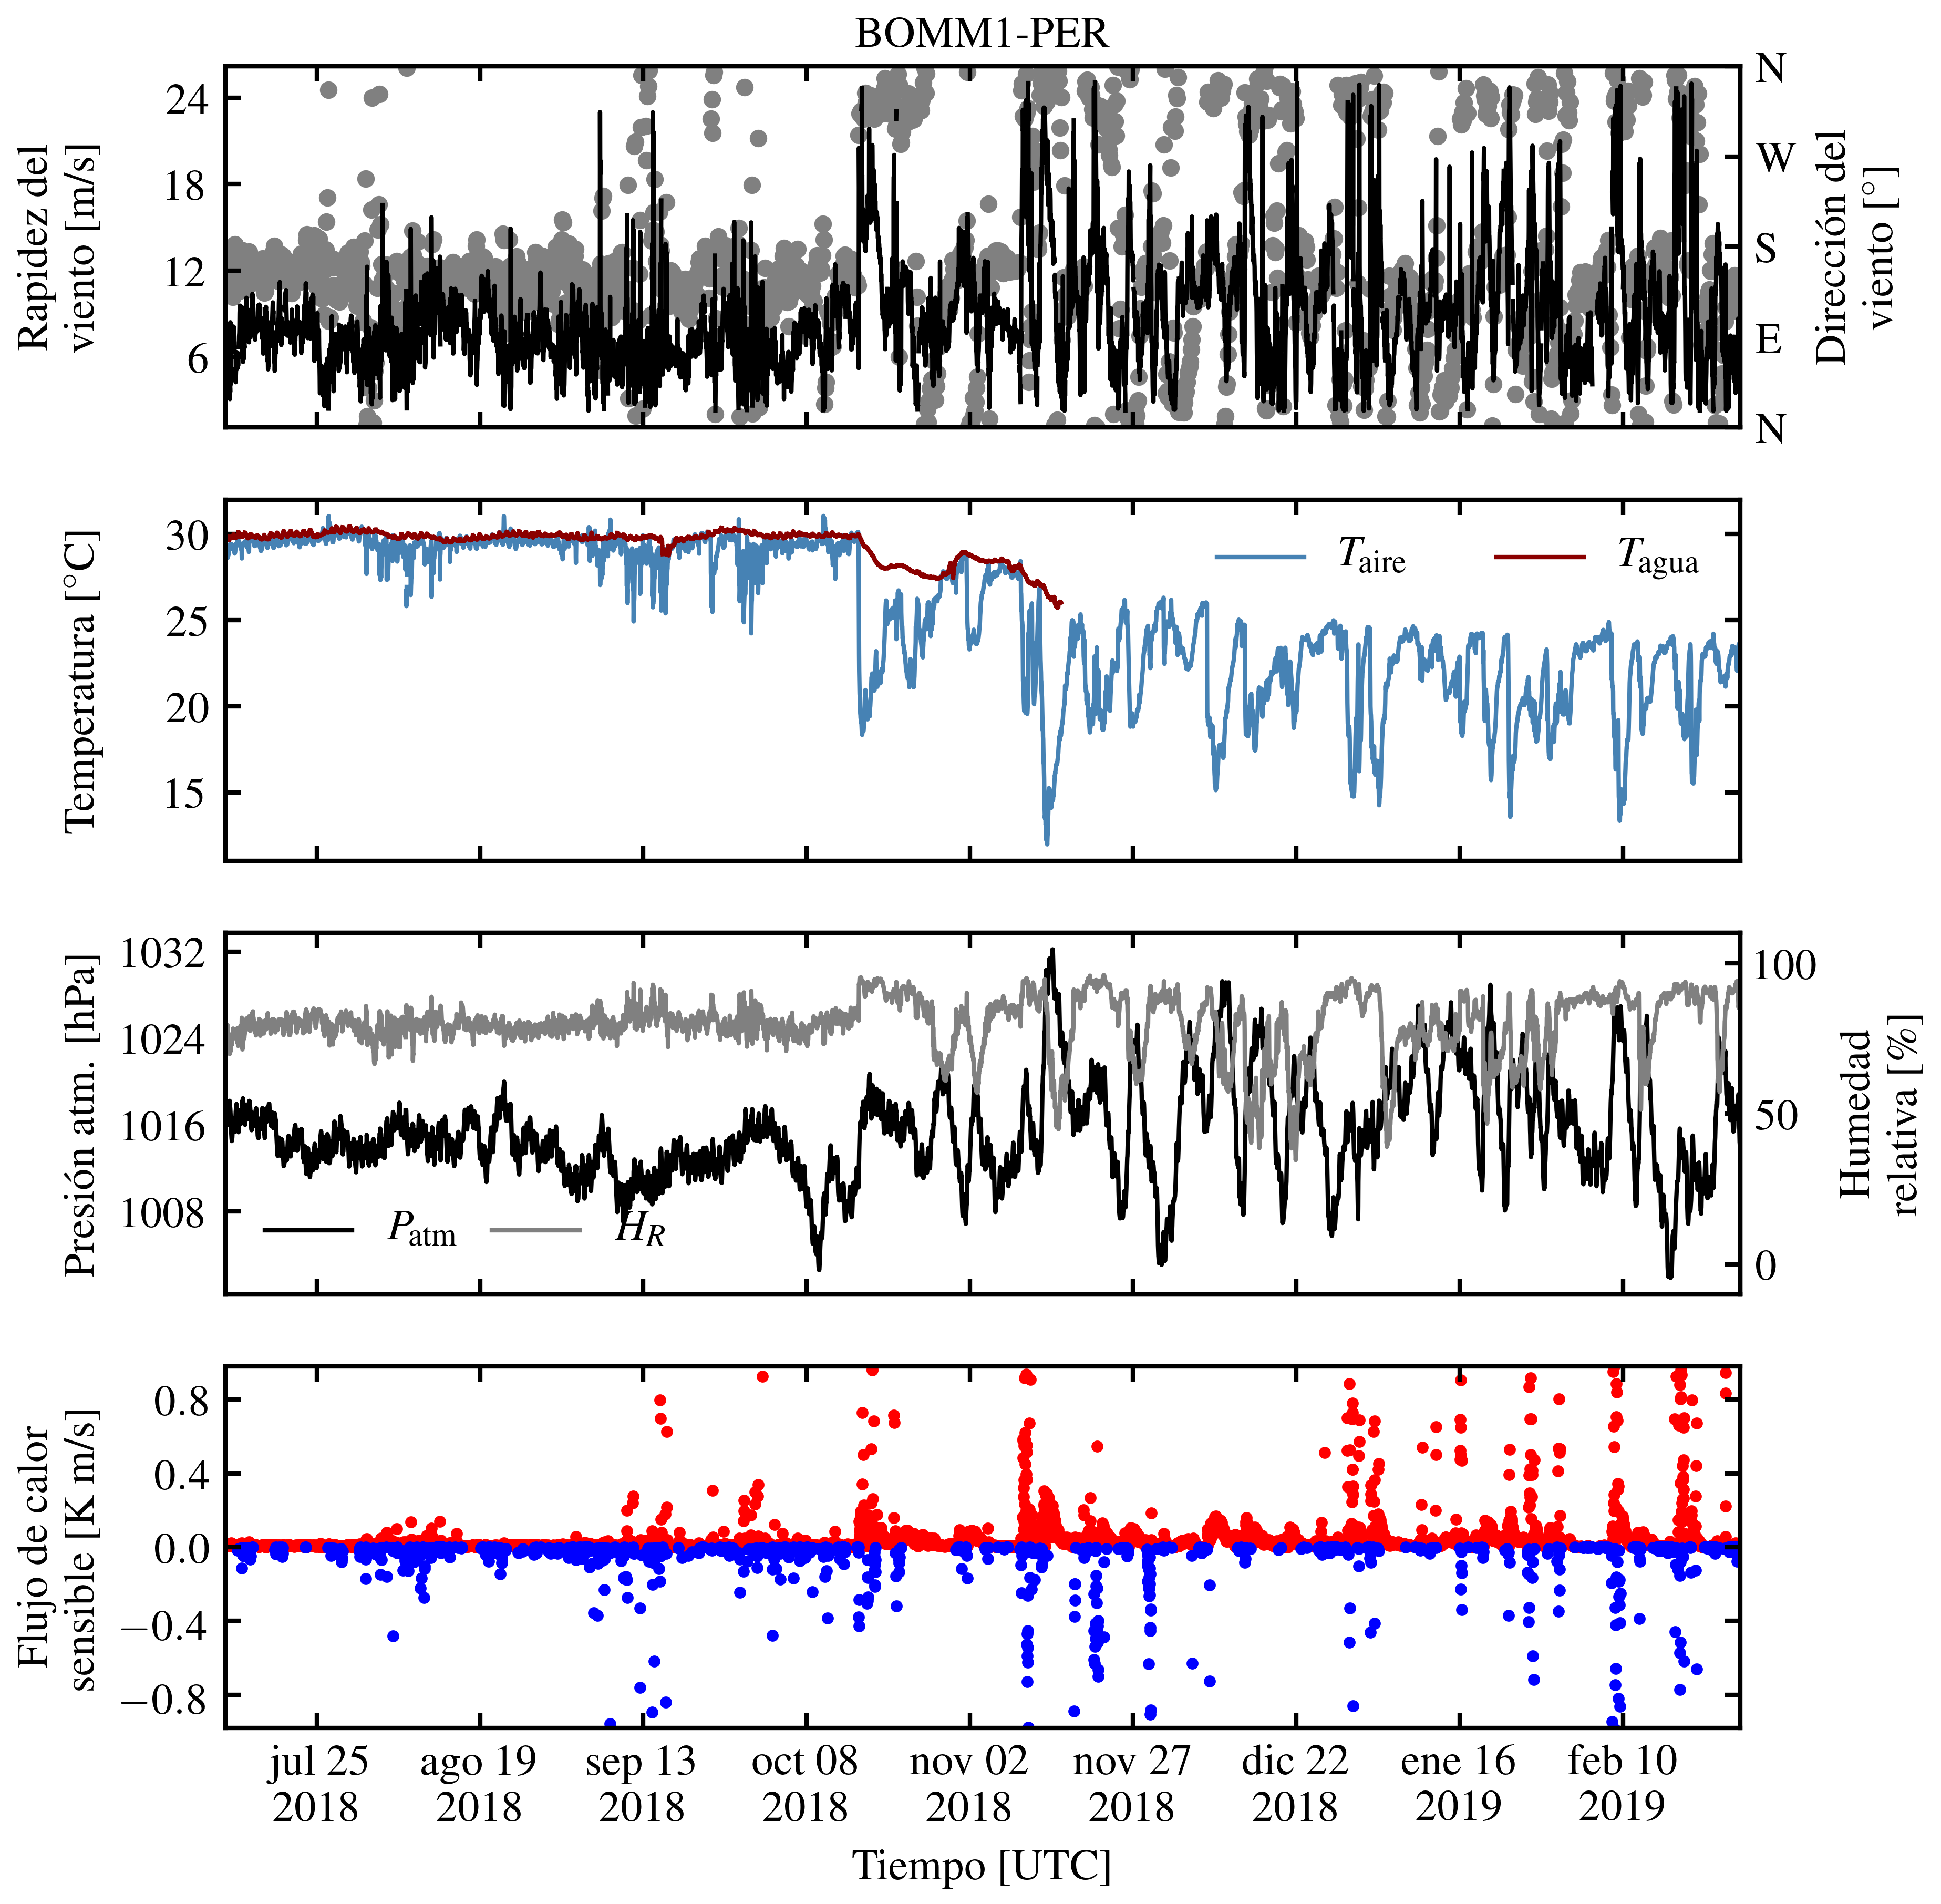
\includegraphics[width=0.85\linewidth]{../figures/bomm1_per_main_variables.png}
  \caption{
    Series de tiempo de las principales variables atmosféricas medidas durante
    el experimento BOMM1-PER en la zona de Perdido, Golfo de México.
  }
  \label{fig:bomm1_per_main_variables}
\end{figure}

Las condiciones del oleaje en el Golfo de México también son bastante diferentes
a las que se presentan en el Pacífico Norte. En la Figura
\ref{fig:bomm1_per_wave_parameters} se puede observar altura significantes que
superan los 4 m, particularmente en la temporada de octubre a febrero, que es
cuando se presentan los Nortes. Debido a que el Golfo de México es una cuenca
semi-cerrada, el crecimiento y desarrollo del oleaje está limitado por el fetch,
por lo tanto, los períodos asociados con el pico espectral que se observaron en
el experimento BOMM1-PER, no superan los 10 s. Tanto en el espectro en
frecuencia del oleaje como en la altura significante, se puede observar una
marcada diferencia entre el período de Nortes y la temporada de verano-otoño. En
esta temporada (de julio a septiembre) se observa un oleaje predominantemente de
baja energía, ya que las alturas de ola no superan los 2 m y los períodos son
del orden de 3 a 5 s en promedio. Adicionalmente, el viento en esta temporada no
superó una rapidez de 10 m/s, exceptuando algunas tormentas localizadas.

\begin{figure}[htpb]
  \centering
  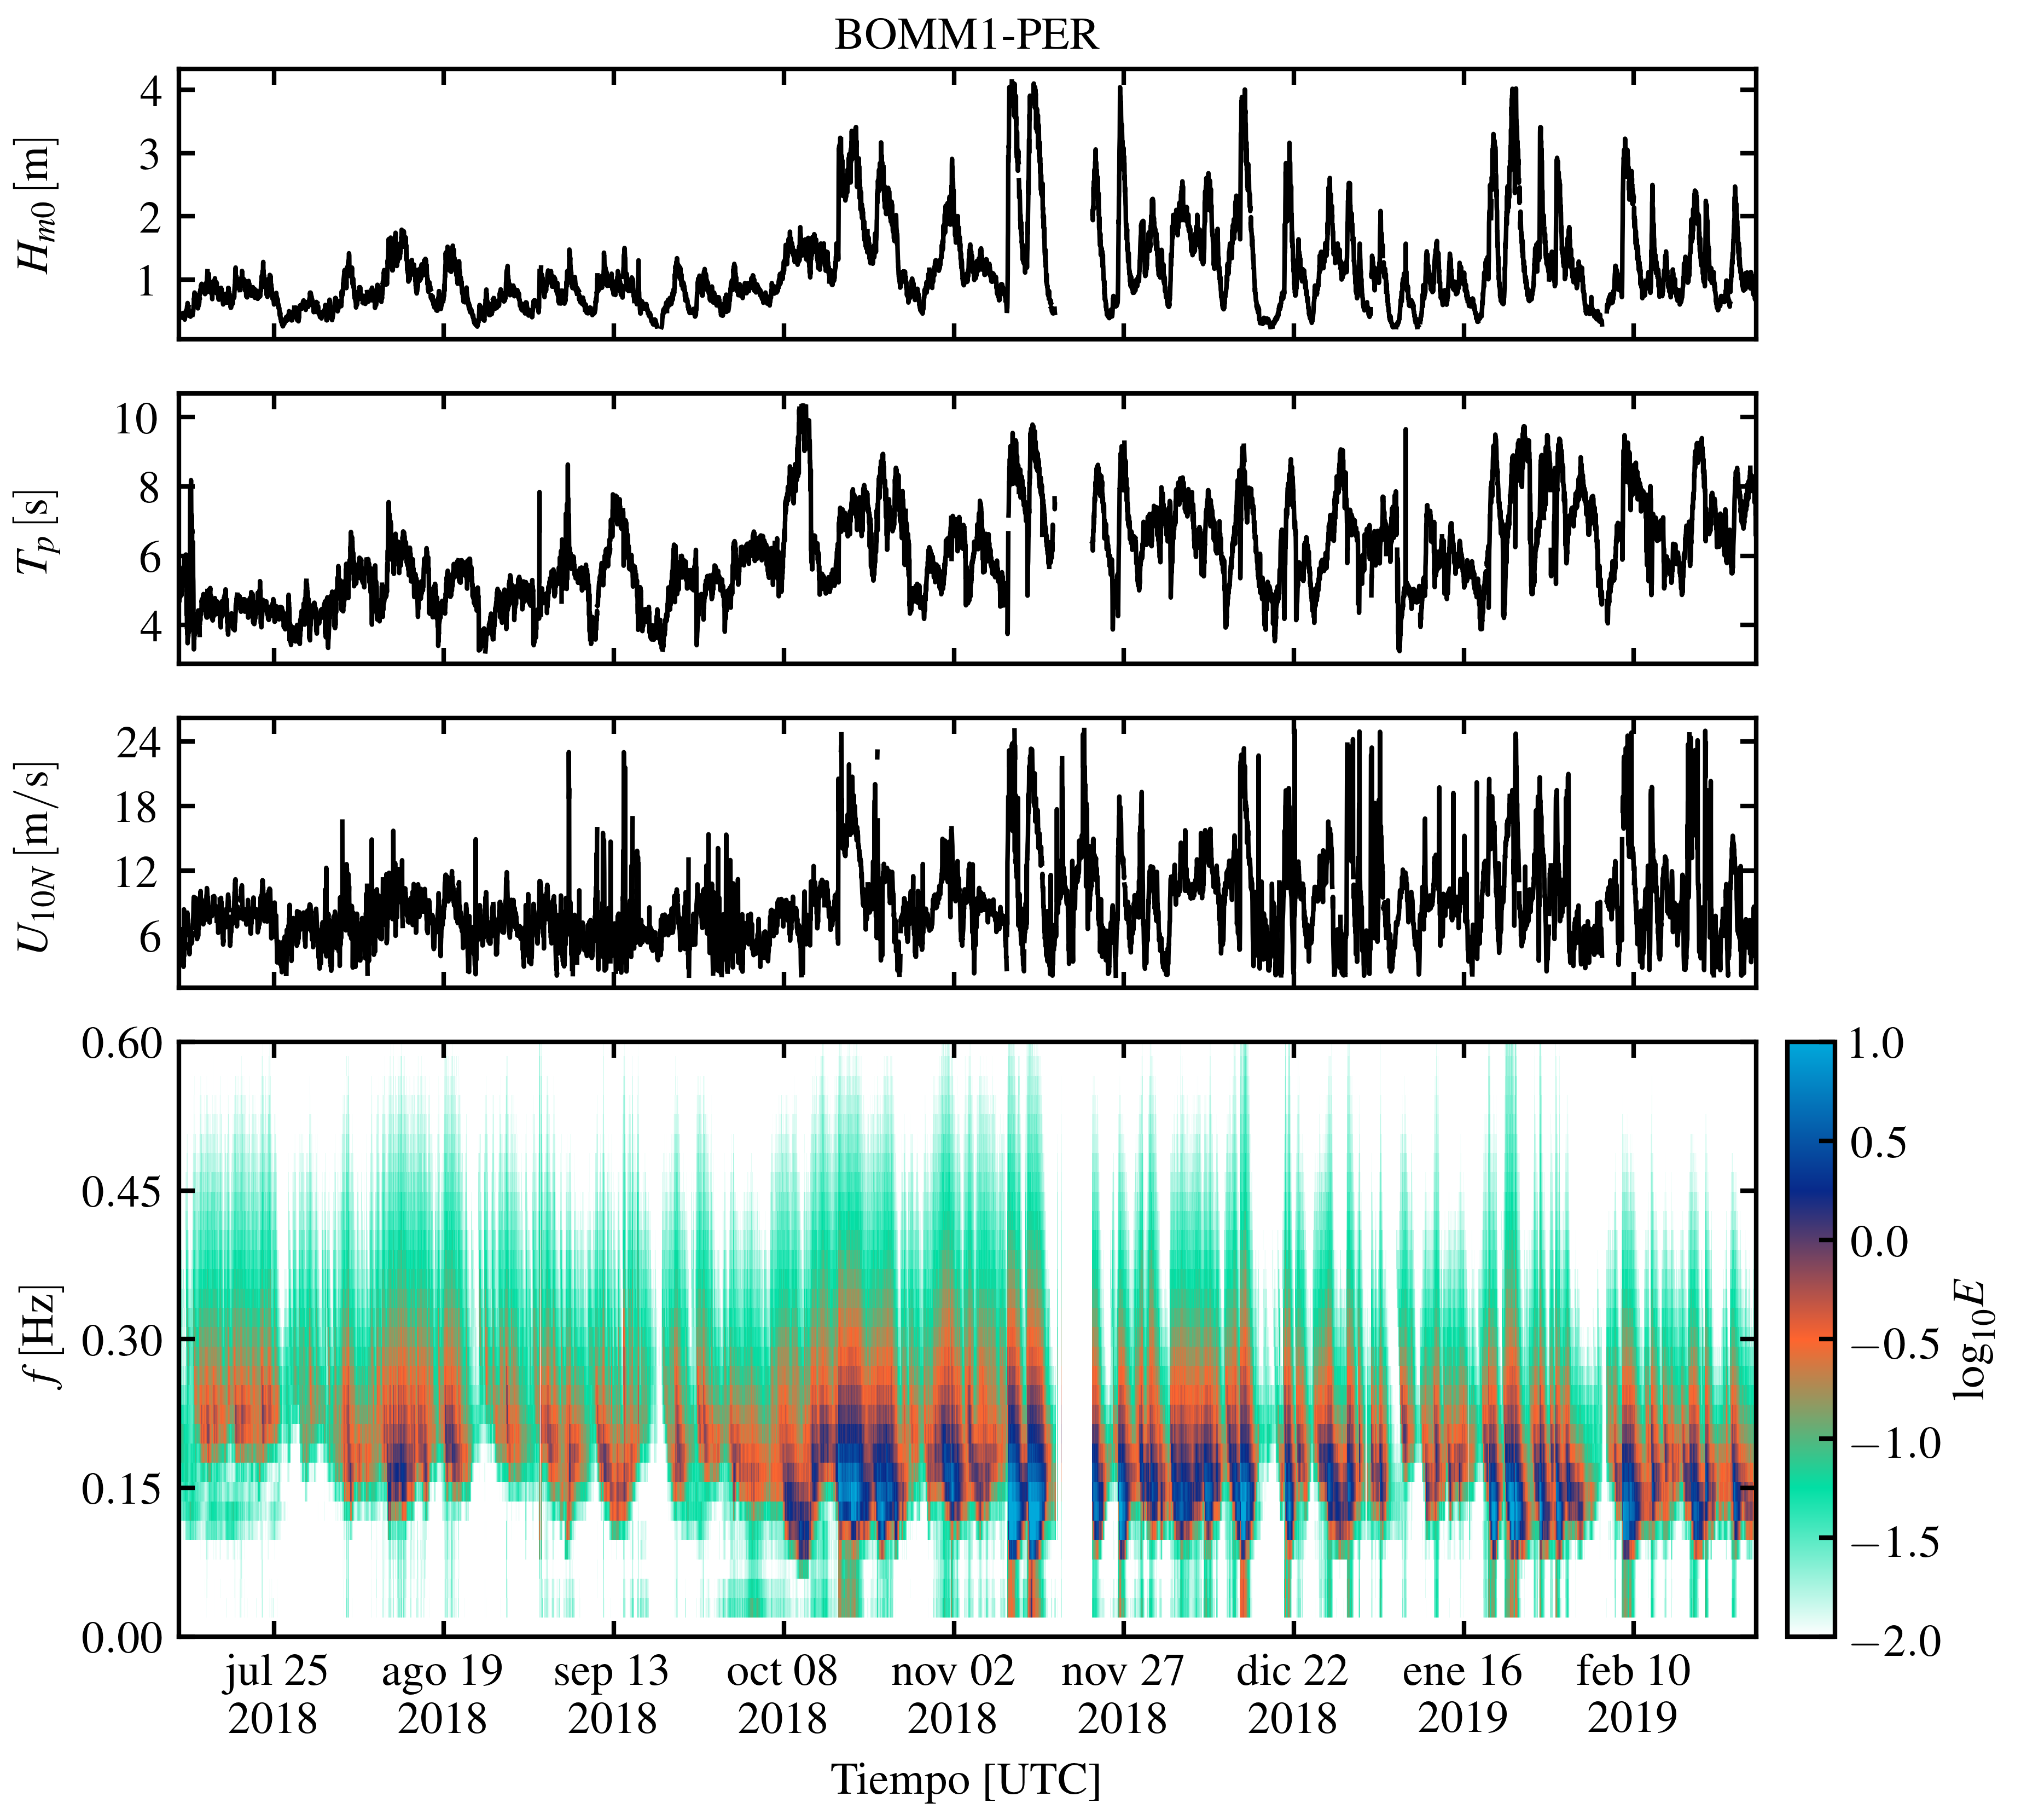
\includegraphics[width=0.85\linewidth]{../figures/bomm1_per_wave_parameters.png}
  \caption{
    Series de tiempo de algunas variables asociadas con el oleaje observadas el
    el experimento BOMM1-PER en la zona de Perdido, Golfo de México.
  }
  \label{fig:bomm1_per_wave_parameters}
\end{figure}

En este caso, el coeficiente de arrastre presenta el mismo comportamiento que en
los experimentos anteriores, a pesar de que se tratan de condiciones diferentes.
En este experimento en particular no se observa una influencia tan directa de la
altura significante en el coeficiente de arrastre, como si se observaba en los
experimentos anteriores. Cabe mencionar que para los datos de BOMM1-PER, debido
a que se presentó una alta variabilidad en los datos, se hizo un control de
calidad más estricto para calcular el coeficiente de arrastre, el cual consistió
en eliminar las velocidades de fricción que superaban 0.8 m/s. A pesar de eso,
se sigue observando una gran variabilidad en $C_D$ cuando la rapidez del viento
es menor de 10 m/s.

\begin{figure}[htpb]
  \centering
  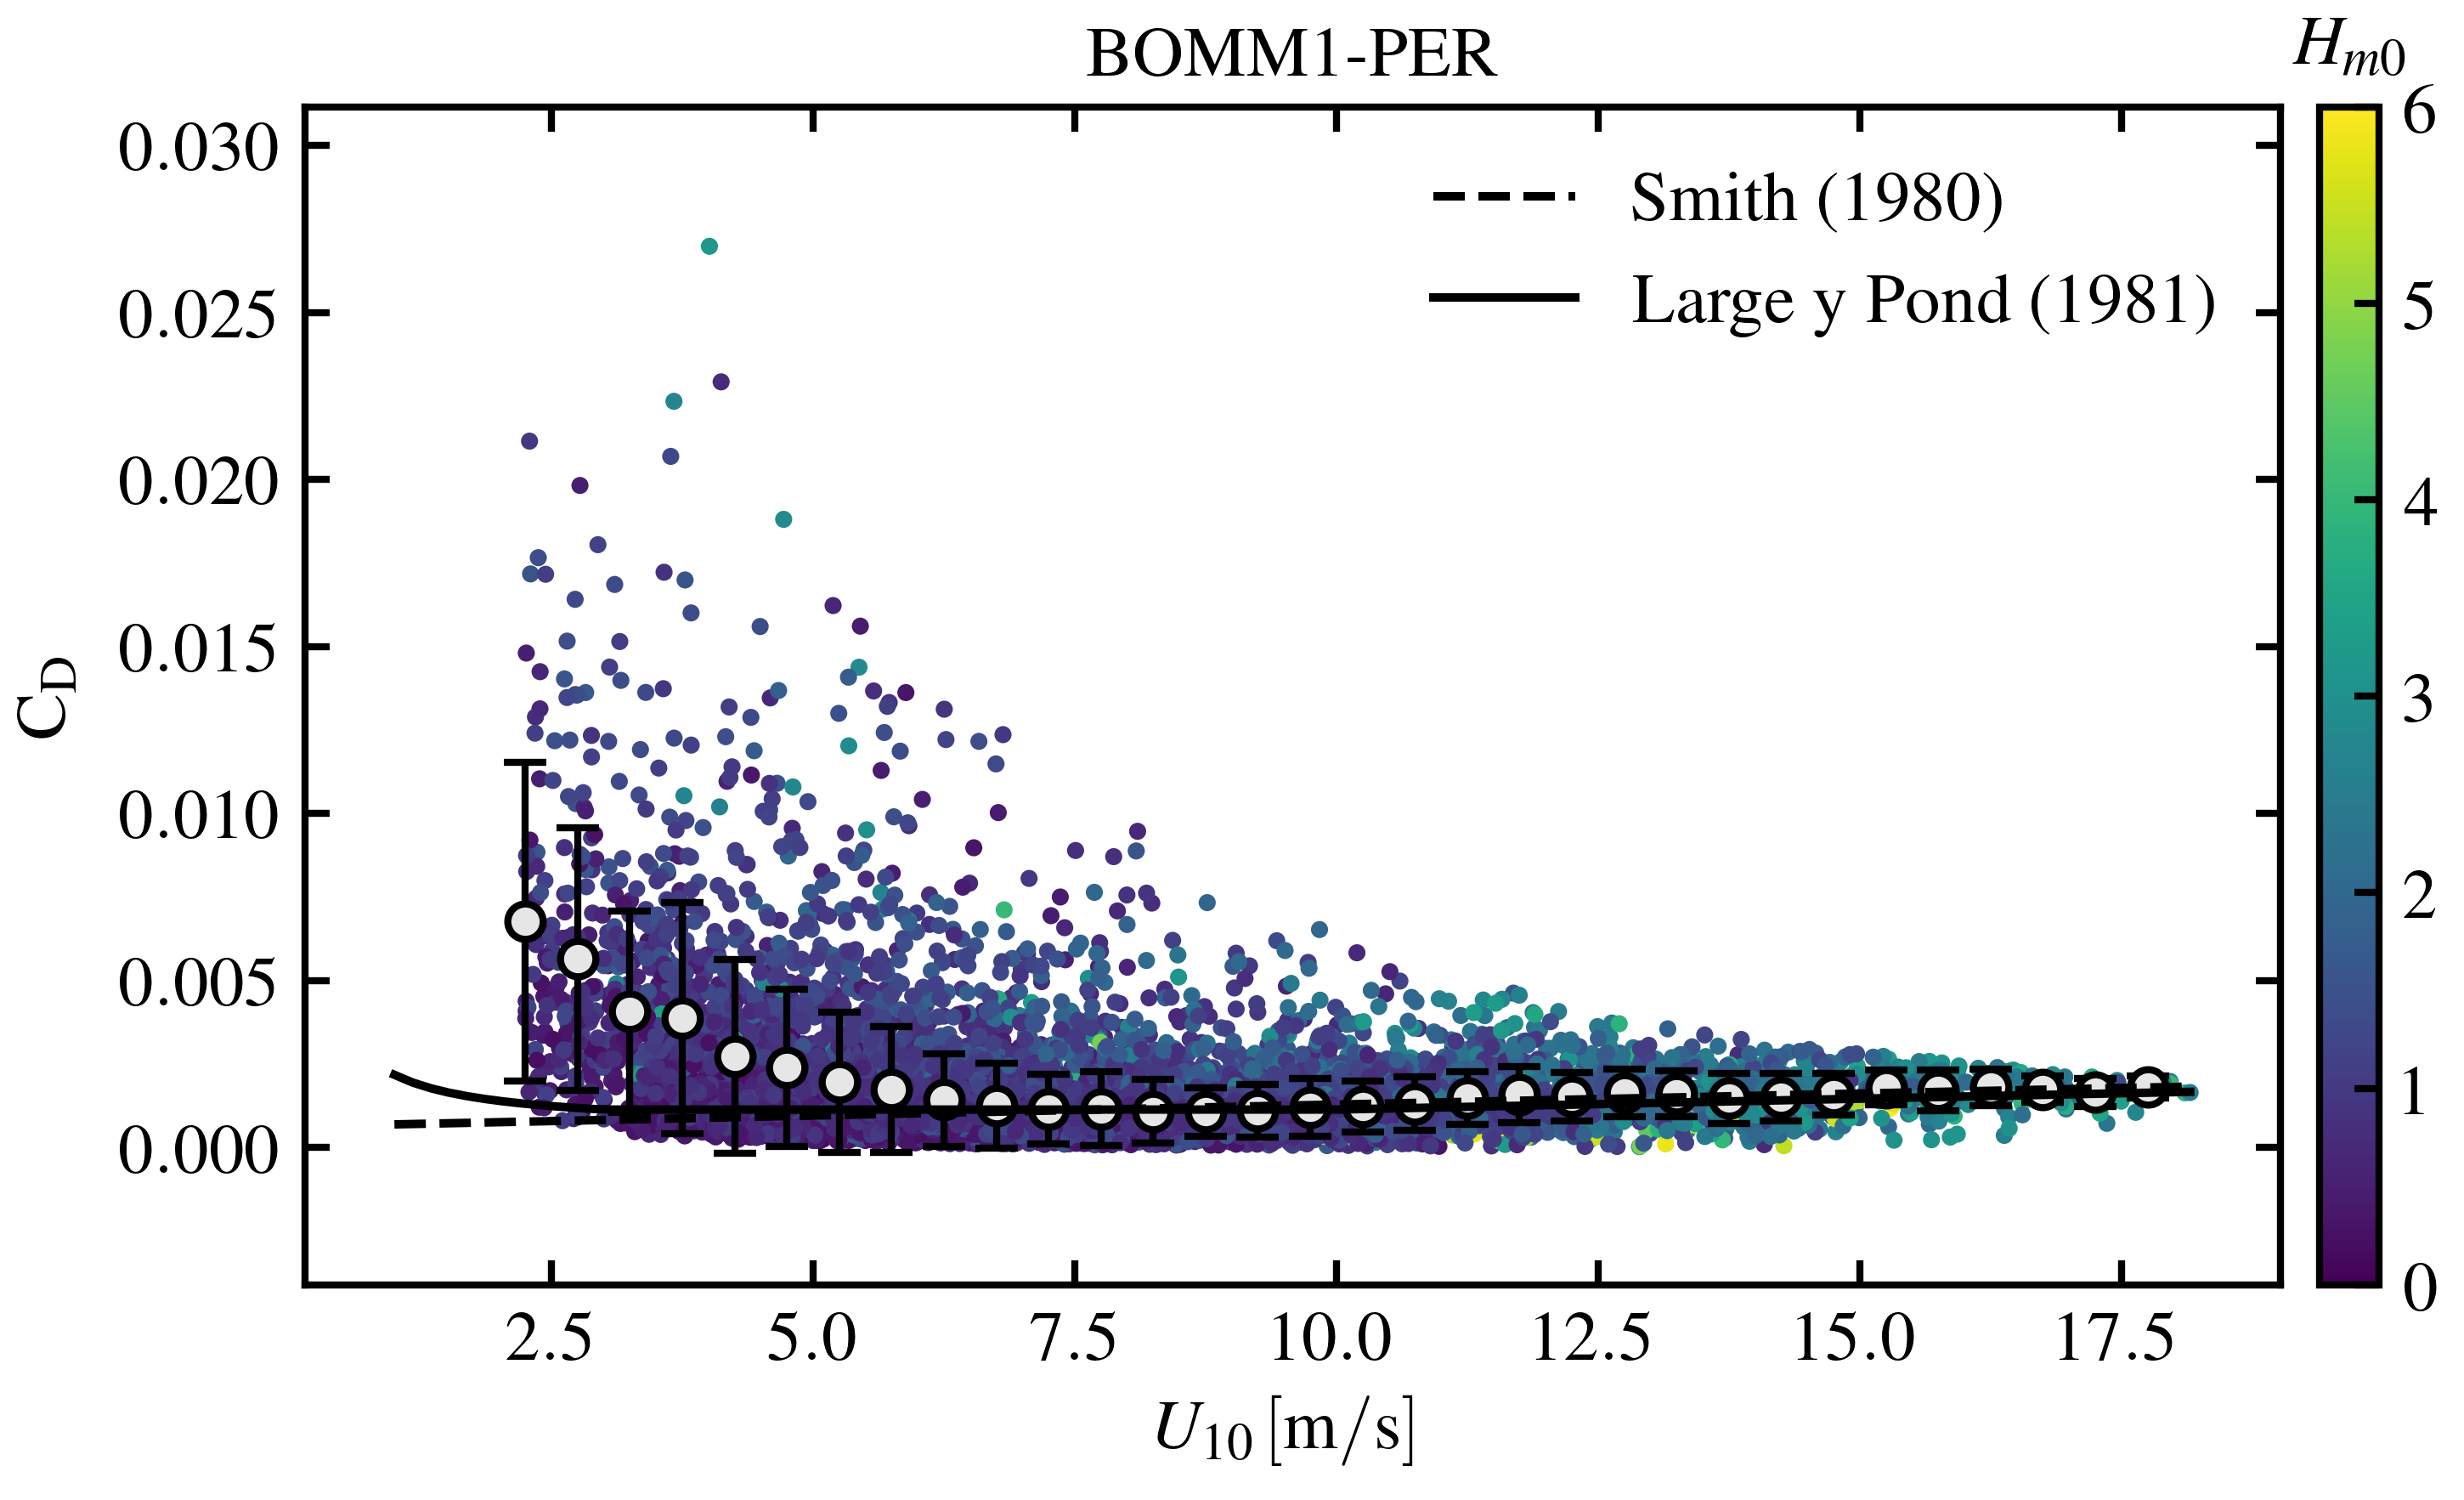
\includegraphics[width=0.68\linewidth]{../figures/bomm1_per_drag_coefficient.png}
  \caption{
    Coeficiente de arrastre en función de la rapidez del viento a 10 metros en
    condiciones neutrales observada durante el experimento BOMM1-PER en la zona
    de Perdido, Golfo de México.  La barra de colores muestra la altura de ola
    significante como indicador del efecto de las olas en el coeficiente de
    arrastre. Las líneas sólida y punteada representan las parametrizaciones de
    \citet{Smith1980} y \citet{LargePond1981}, respectivamente. Los puntos
    blancos con borde negro representan los promedios de $C_D$ para 20
    intervalos de clase de $U_{10}$ y las barras representan la desviación
    estándar de cada intervalo.
  }
  \label{fig:bomm1_per_drag_coefficient}
\end{figure}

Finalmente, la diferencia entre las direcciones del viento en BOMM1-PER, se
asemejan mucho a la del experimento BOMM2-ITS, ya que se presenta un sesgo de
aproximadamente $3-4^\circ{}$, como se observa en la Figura
\ref{fig:bomm1_per_wind_direction_histogram}.

\begin{figure}[t]
  \centering
  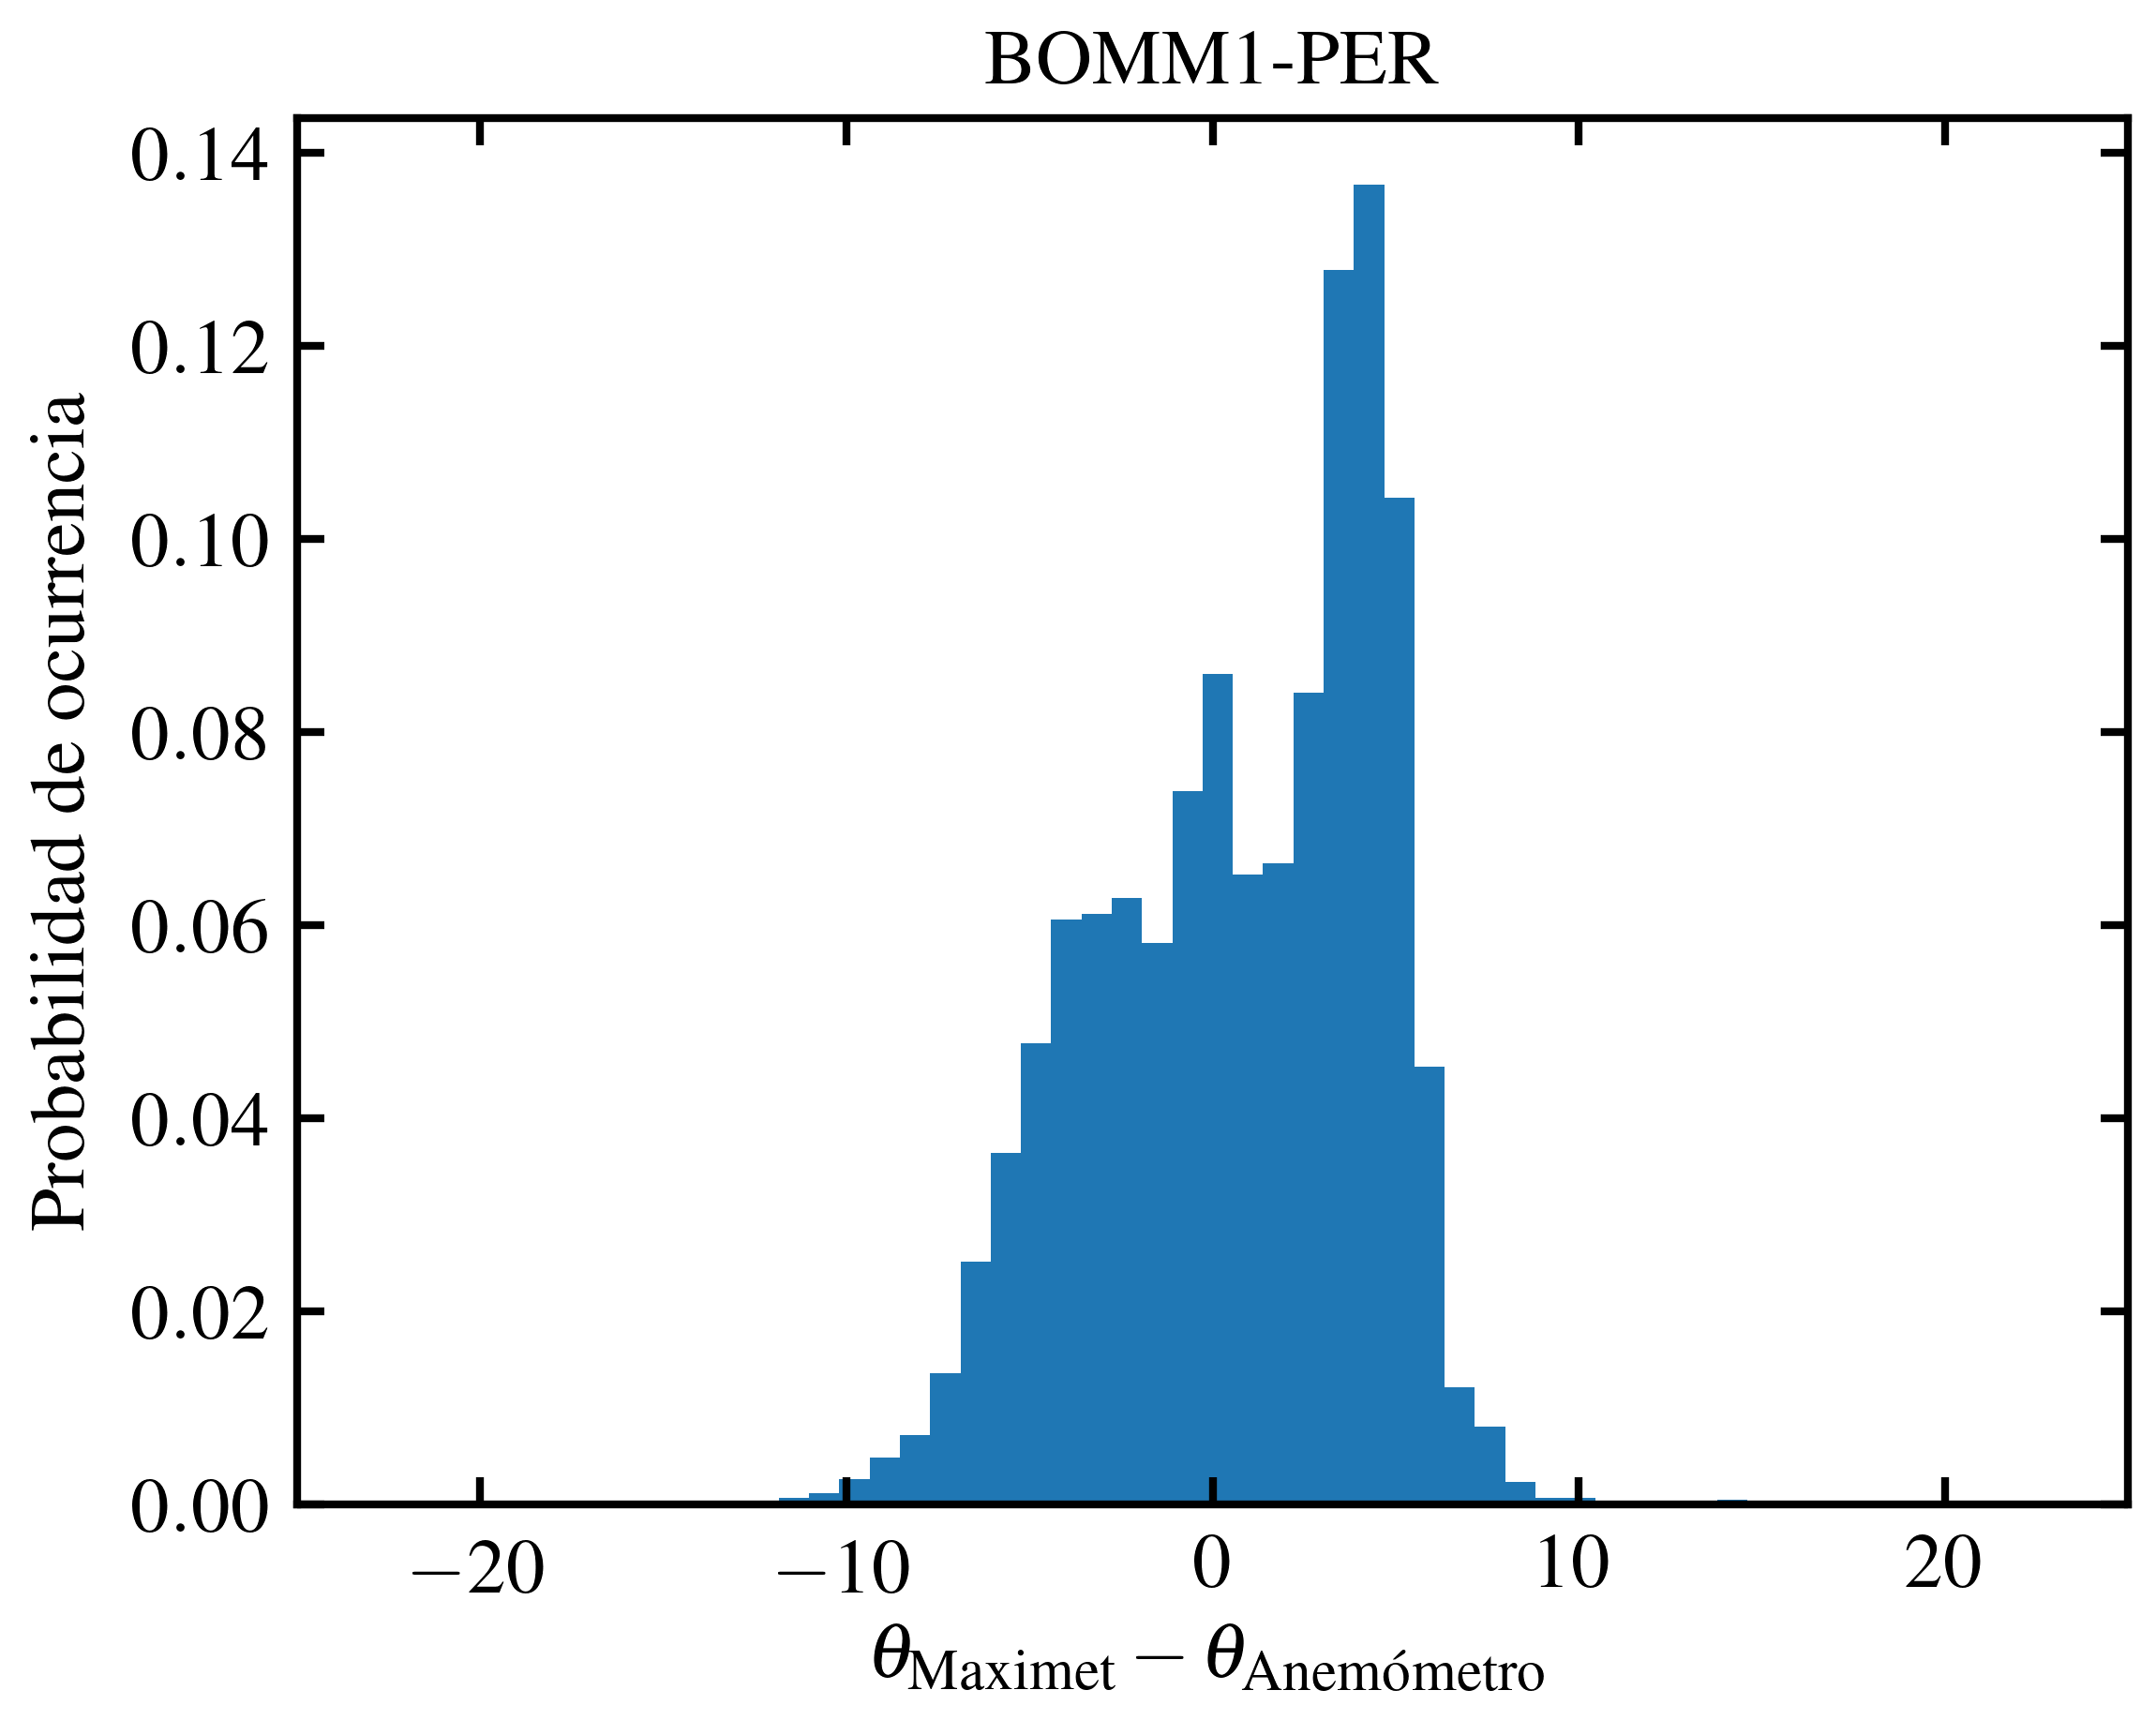
\includegraphics[width=0.5\linewidth]{../figures/bomm1_per_wind_direction_histogram.png}
  \caption{
    Histograma de la diferencia entre la dirección del viento real observada con
    la estación meteorológica Maximet y la dirección del viento calculada del
    anemómetro sónico después de aplicar la corrección de los datos por el
    movimiento de la boya. Los datos corresponden a las observaciones llevadas a
    cabo durante el experimento BOMM1-ITS en las inmediaciones de la Isla Todos
    Santos, Ensenada, BC.
  }
  \label{fig:bomm1_per_wind_direction_histogram}
\end{figure}


% }}}

% }}}

% comentarios finales {{{
\clearpage
\section{Comentarios finales}
\label{sec:comentarios_finales}

La instalación de esta red de boyas hace parte del proyecto
financiado por CONACYT y por la Secretaría de Energía (SENER), y es llevado a
cabo por el Consorcio de Investigación del Golfo de México (CIGoM) dentro de la
Línea de Acción 1, ``Plataformas de observación oceanográfica'', en
colaboración con la Secretaría de Marina (SEMAR).

En este reporte se presentan los principales resultados obtenidos del análisis
de los datos observados con la Boyas Oceanográficas y de Meteorología Marina
(BOMM), tanto en sus períodos de prueba como en la Isla Todos Santos, como en su
períodos de operación en el Golfo de México.

Con estas mediciones se pretende obtener información suficiente para determinar
las características y la variabilidad de los fenómenos físicos dominantes en las
regiones costeras del Golfo de México, enfocados en procesos de interacción
entre el océano y la atmósfera, particularmente los flujos de momentum y las
características del espectro direccional del oleaje.

Los datos presentados en este reporte constituyen un análisis preliminar, por lo
tanto es importante considerar que aún se debe realizar un procesamiento más
detallado y un análisis profundo de los datos antes de presentar resultados
contundentes. La información contenida en este reporte se encuentra aun bajo
procesamiento y control de calidad.

% }}}

% referencias {{{
\clearpage
\bibliographystyle{apalike}
\nocite{*}
\bibliography{./references.bib}
% }}}


\end{document}
%  finalizar documento --------------------------------------------------------
